\documentclass{article}


\usepackage[utf8]{inputenc}
\usepackage[english]{babel}
\usepackage{authblk,url}
\usepackage{amssymb,amsmath,amsthm,twoopt,xargs,mathtools,dsfont}
\usepackage{times,ifthen}
\usepackage{fancyhdr,xcolor}
\usepackage{hyperref}

\newtheorem{axiom}{Axiom}
\newtheorem{remark}{Remark}
\newtheorem{claim}[axiom]{Claim}
\newtheorem{theorem}{Theorem}[section]
\newtheorem{lemma}[theorem]{Lemma}
\newtheorem{proposition}[theorem]{Proposition}
\newtheorem{corollary}[theorem]{Corollary}

\title{Backward variational inference and application to noisy Independent Component Analysis}
\date{}

%\author[$\wr$]{Mathis Chagneux}
\author[$\dag$]{XXX}
%\affil[$\wr$]{{\small LTCI, T\'el\'ecom Paris, Institut Polytechnique de Paris, Palaiseau.}}

\affil[$\dag$]{{\small }}

\lhead{}
\rhead{}

\DeclareUnicodeCharacter{2212}{-}
\usepackage{geometry}
\pagestyle{fancy}


\newcommand{\retrokmodnorm}{\bar{\boldsymbol{\mathcal{L}}}^{\precpar,\theta}}
\newcommand{\xarb}{x^\ast}
\newcommand{\precparsp}{\mathcal{E}}
\newcommand{\fk}[2]{\mathbf{F}_{#1 | #2}}
\newcommand{\probmeas}[1]{\mathsf{M}_1(#1)}
\newcommand{\Xfd}{\mathcal{X}}
\newcommand{\uksymbol}{\ell}
\newcommandx{\bkmod}[2][1=]{ 
\ifthenelse{\equal{#1}{}}
{\kernel{B}_{#2}^\precpar}
{\kernel{B}_{#2}^\precpar}
}

\newcommand{\cev}[1]{\reflectbox{\ensuremath{\vec{\reflectbox{\ensuremath{#1}}}}}}
\newcommand{\ukmod}[1]{\mathbf{L}_{#1}^\precpar}
\newcommand{\shiftbwd}{\cev{\shiftsymbol}^{\precpar}}
\newcommand{\shiftfwd}{\vec{\shiftsymbol}^{\, \precpar}}
\newcommand{\shiftsymbol}{\Phi}
\newcommand{\precpar}{\varphi}
\newcommand{\intvect}[2]{\{ #1, #2 \}}
\newcommandx\tstatmod[2][1=]{
\ifthenelse{\equal{#1}{}}
	{\tstatletter^{\precpar}_{#2}}
	{\tau^{\precpar}_{#2}^{#1}}
}
\newcommand{\noshift}{\shiftsymbol^{\precpar}}
\newcommand{\udlow}{\sigma_-}
\newcommand{\udup}{\sigma_+}
\newcommand{\retrok}{\boldsymbol{\mathcal{L}}}
%\newcommand{\intvect}[2]{\llbracket #1, #2 \rrbracket}
\newcommandx{\bkw}[2][1=]{ 
\ifthenelse{\equal{#1}{}}
{\kernel{B}_{#2}}
{\kernel{B}_{#2}}
}
\newcommand{\retroknorm}{\bar{\boldsymbol{\mathcal{L}}}}
\newcommand{\ud}[1]{\uksymbol_{#1}} 
\newcommand{\nset}{\mathbb{N}}
\newcommand{\nsetpos}{\mathbb{N}_{> 0}}
\newcommand{\1}{\mathbbm{1}} 
\newcommandx{\postmod}[2][1=]{
\ifthenelse{\equal{#1}{}}
	{\phi_{#2}^\varphi}
	{\phi_{#2}^\N}
}
\newcommand{\retrokmod}{\boldsymbol{\mathcal{L}}^{\precpar,\theta}}
\newcommand{\uk}[1]{\mathbf{L}_{#1}}
\newcommand{\tensprod}{\otimes}
\def\dimX{d}
\def\dimY{m}
%\def\Xset{\mathsf{X}}
\newcommand{\Xset}{\mathsf{X}}
\def\Yset{\mathsf{Y}}
\newcommand{\mk}{\kernel{G}}
\newcommand{\hk}{\kernel{Q}}
\newcommand{\md}[1]{g_{#1}}
\newcommand{\SmoothFigSize}{0.27}

\newcommand{\logllh}[1]{\ell_{#1}}
\newcommand{\llh}[1]{\mathsf{L}_{#1}}
\newcommand{\testf}{\mathsf{h}}

\newcommandx\filtderiv[2][1=]{
\ifthenelse{\equal{#1}{}}
	{\eta_{#2}}
	{\eta_{#2}^\N}
}
\newcommand{\pred}[1]{\pi_{#1}}
\newcommand{\parvec}{\theta}
\newcommand{\parspace}{\Theta}
\newcommand{\tstatletter}{\kernel{T}}
%\newcommand{\retrok}{\kernel{D}}
\newcommandx\tstat[2][1=]{
\ifthenelse{\equal{#1}{}}
	{\tstatletter_{#2}}
	{\tau_{#2}^{#1}}
}
\newcommandx\tstathat[2][1=]{
\ifthenelse{\equal{#1}{}}
	{\tstatletter_{#2}}
	{\widehat{\tau}_{#2}^{#1}}
}
\newcommand{\af}[1]{h_{#1}}
\newcommand{\deriv}{\nabla_{\parvec}}

\newcommand{\kernel}[1]{\mathbf{#1}}
\newcommand{\bmf}[1]{\set{F}(#1)}
\newcommand{\set}[1]{\mathsf{#1}}

\newcommandx{\bk}[2][1=]{
\ifthenelse{\equal{#1}{}}
{\overleftarrow{\kernel{Q}}_{#2}}
{\overleftarrow{\kernel{Q}}_{#2}^{#1}}
}

\newcommandx{\bkhat}[2][1=]{
\ifthenelse{\equal{#1}{}}
{\widehat{\kernel{Q}}_{#2}}
{\widehat{\kernel{Q}}_{#2}^{#1}}
}

\newcommand{\lk}{\kernel{L}}
\newcommand{\idop}{\operatorname{id}}
\newcommand{\hd}[1]{q_{#1}}
\newcommand{\hdhat}[1]{\widehat{q}_{#1}}


\newcommandx{\addf}[2][1=]{
\ifthenelse{\equal{#1}{}}{\termletter_{#2}}{\bar{h}_{#2 | #1}}
}
\newcommand{\addfc}[1]{\underline{\termletter}_{#1}}
\newcommand{\adds}[1]{\af{#1}}
\newcommand{\term}[1]{\termletter_{#1}}
\newcommand{\termletter}{\tilde{h}}
\newcommand{\N}{N}
\newcommand{\partpred}[1]{\pi_{#1}^\N}
\newcommand{\tstattil}[2]{\tilde{\tau}_{#2}^{#1}}
\newcommandx{\K}[1][1=]{
\ifthenelse{\equal{#1}{}}{{\kletter}}{{\widetilde{\N}^{#1}}}}
\newcommand{\hkup}{\bar{\varepsilon}}
\newcommand{\bi}[3]{J_{#1}^{(#2, #3)}}
\newcommand{\bihat}[3]{\widehat{J}_{#1}^{(#2, #3)}}

\newcommand{\kletter}{\widetilde{\N}}

\def\sigmaX{\mathcal{X}}
\def\sigmaY{\mathcal{Y}}
\def\1{\mathds{1}}
\def\pE{\mathbb{E}}
\def\pP{\mathbb{P}}
\def\plim{\overset{\pP}{\longrightarrow}}
\def\dlim{\Longrightarrow}
\def\gauss{\mathcal{N}}


\newcommand{\esssup}[2][]
{\ifthenelse{\equal{#1}{}}{\left\| #2 \right\|_\infty}{\left\| #2 \right\|^2_{\infty}}}


\newcommand{\swght}[2]{\ensuremath{\omega_{#1}^{#2}}}

\newtheorem{assumptionA}{\textbf{A}\hspace{-3pt}}
\newcommand{\rset}{\ensuremath{\mathbb{R}}}
\newcommand{\iid}{i.i.d.}

\newcommand{\smwght}[3]{\tilde{\omega}_{#1|#2}^{#3}}
\newcommand{\smwghtfunc}[2]{\tilde{\omega}_{#1|#2}}

\newcommand{\smpart}[3]{\ensuremath{\tilde{\xi}_{#1|#2}^{#3}}}
\def\aux{{\scriptstyle{\mathrm{aux}}}}
\newcommand{\bdm}{\mathsf{TwoFilt}_{bdm}}
\newcommand{\fwt}{\mathsf{TwoFilt}_{fwt}}

\newcommand{\kiss}[3][]
{\ifthenelse{\equal{#1}{}}{r_{#2|#3}}
{\ifthenelse{\equal{#1}{fully}}{r^{\star}_{#2|#3}}
{\ifthenelse{\equal{#1}{smooth}}{\tilde{r}_{#2|#3}}{\mathrm{erreur}}}}}

\newcommand{\chunk}[4][]%
{\ifthenelse{\equal{#1}{}}{\ensuremath{{#2}_{#3:#4}}}{\ensuremath{#2^#1}_{#3:#4}}
}

\newcommand{\kissforward}[3][]
{\ifthenelse{\equal{#1}{}}{p_{#2}}
{\ifthenelse{\equal{#1}{fully}}{p^{\star}_{#2}}
{\ifthenelse{\equal{#1}{smooth}}{\tilde{r}_{#2}}{\mathrm{erreur}}}}}

\newcommand{\instrpostaux}[1]{\ensuremath{\upsilon_{#1}}}
\newcommandx\post[2][1=]{
\ifthenelse{\equal{#1}{}}
	{\phi_{#2}}
	{\phi_{#2}^\N}
}

\newcommandx\posthat[2][1=]{
\ifthenelse{\equal{#1}{}}
	{\widehat{\phi}_{#2}}
	{\widehat{\phi}_{#2}^\N}
}

\newcommand{\adjfunc}[4][]
{\ifthenelse{\equal{#1}{}}{\ifthenelse{\equal{#4}{}}{\vartheta_{#2|#3}}{\vartheta_{#2|#3}(#4)}}
{\ifthenelse{\equal{#1}{smooth}}{\ifthenelse{\equal{#4}{}}{\tilde{\vartheta}_{#2|#3}}{\tilde{\vartheta}_{#2|#3}(#4)}}
{\ifthenelse{\equal{#1}{fully}}{\ifthenelse{\equal{#4}{}}{\vartheta^\star_{#2|#3}}{\vartheta^\star_{#2|#3}(#4)}}{\mathrm{erreur}}}}}

\newcommand{\XinitIS}[2][]
{\ifthenelse{\equal{#1}{}}{\ensuremath{\rho_{#2}}}{\ensuremath{\check{\rho}_{#2}}}}
\newcommand{\adjfuncforward}[1]{\vartheta_{#1}}
\newcommand{\rmd}{\ensuremath{\mathrm{d}}}
\newcommand{\eqdef}{\ensuremath{:=}}
\newcommand{\eqsp}{\;}
\newcommand{\ewght}[2]{\ensuremath{\omega_{#1}^{#2}}}
\newcommand{\ewghthat}[2]{\ensuremath{\widehat{\omega}_{#1}^{#2}}}
\newcommand{\epart}[2]{\ensuremath{\xi_{#1}^{#2}}}
\newcommand{\filt}[2][]%
{%
\ifthenelse{\equal{#1}{}}{\ensuremath{\phi_{#2}}}{\ensuremath{\phi_{#1,#2}}}%
}
\newcommand{\Xinit}{\ensuremath{\chi}}
\newcommand{\sumwght}[2][]{%
\ifthenelse{\equal{#1}{}}{\ensuremath{\Omega_{#2}}}{\ensuremath{\Omega_{#2}^{(#1)}}}}
\newcommand{\sumwghthat}[2][]{%
\ifthenelse{\equal{#1}{}}{\ensuremath{\widehat{\Omega}_{#2}}}{\ensuremath{\widehat{\Omega}_{#2}^{(#1)}}}}

\newcounter{hypH}
\newenvironment{hypH}{\refstepcounter{hypH}\begin{itemize}
\item[{\bf H\arabic{hypH}}]}{\end{itemize}}

\newcommand{\marginalset}{\mathsf{U}}

\newcommand{\calF}[2]{\mathcal{F}_{#1}^{#2}}
\newcommand{\calG}[2]{\mathcal{G}_{#1}^{#2}}
\newcommand{\Uset}{\mathsf{U}}
\newcommand{\tcalF}[2]{\widetilde{\mathcal{F}}_{#1}^{#2}}
\newcommand{\tcalG}[2]{\widetilde{\mathcal{G}}_{#1}^{#2}}

\newcommand{\kernelmarg}{\mathbf{R}}

\newcommand{\pplim}{\overset{\pP}{ \underset{\N \to \infty}{\longrightarrow}}}
\newcommand{\ddlim}{\overset{\mathcal{D}}{ \underset{\N \to \infty}{\longrightarrow}}}
\newcommand{\aslim}{\overset{\pP\mathrm{-a.s.}}{ \underset{\N \to \infty}{\longrightarrow}}}

\newcommand{\qg}[1]{\ell_{#1}}
\newcommand{\hatqg}[1]{\mathsf{\ell}_{#1}}

\newcommand{\sfd}{\mathsf{d}}
\newcommand{\X}{\mathbf{X}}
\newcommand{\x}{\mathbf{x}}
\newcommand{\y}{\mathbf{y}}
\newcommand{\E}{\mathbb{E}}
\newcommand{\e}{\text{e}}
\newcommand{\W}{\mathbf{W}}
\newcommand{\Z}{\mathbf{Z}}
\newcommand{\frob}{:}
\newcommand{\rme}{\mathrm{e}}
\newcommand{\vois}{\mathcal{V}}




\newcounter{example}[section]
\newenvironment{example}[1][]{\refstepcounter{example}\par\medskip
   \noindent \textbf{Example~\theexample:} \textit{#1} \text \rmfamily}{\medskip}

\newcommand{\expect}[2]{\mathbb{E}_{#1}\left[#2\right]}
\newcommand{\gaussian}[2]{\mathcal{N}\left( #1, #2 \right)}
\newcommand{\backward}[1]{\overleftarrow{#1}}
\newcommand{\vbackward}[1]{q_{1:#1}(z_{#1}|z_{#1 + 1})}
\newcommand{\vfilt}[1]{q_{1:#1}(z_{#1})}
\newcommand{\vbackwardparam}[2]{\backward{#1}_{1:#2}^\phi}
\newcommand{\vbackwardmean}[1]{\vbackwardparam{\mu}{#1}}
\newcommand{\vbackwardcov}[1]{\vbackwardparam{\Sigma}{#1}}
\newcommand{\vfiltparam}[2]{#1_{1:#2}^\phi}
\newcommand{\vfiltmean}[1]{\vfiltparam{\mu}{#1}}
\newcommand{\vfiltcov}[1]{\vfiltparam{\Sigma}{#1}}
\newcommand{\inv}[1]{{#1}^{-1}}
\newcommand{\stateprec}{\inv{Q^\theta}}
\newcommand{\vstateprec}{\inv{Q^\phi}}
\newcommand{\quadform}[2]{#1^T #2 #1}


\DeclareMathOperator*{\argmax}{arg\,max} 

\begin{document}

\maketitle

\begin{abstract}

\end{abstract}

\section{Introduction}

\section{Latent data models and backward variational inference}
Let $\parvec$ be a parameter lying in a $\Theta\subset \rset^q$ and consider a  \textit{state space model} where the hidden Markov chain  in $\rset^d$ is denoted by $(X_k)_{k\geqslant 0}$. The distribution of $X_0$ has density $\chi_\theta$ with respect to the Lebesgue measure $\mu$ and for all $0\leqslant k \leqslant n-1$, the conditional distribution of $X_{k+1} $ given $X_{0:k}$ has density $\hd{k+1;\parvec}(X_{k},\cdot)$, where $a_{u:v}$ is a short-hand notation for $(a_u,\ldots,a_v)$. 
It is assumed that this state  is partially observed  through an observation process $(Y_k)_{0\leqslant k \leqslant n}$ taking values in $\rset^m$. 
For all $0\leqslant k \leqslant n$, the distribution of $Y_k$ given $X_{0:n}$ depends on $X_k$ only and has density $\md{k;\parvec}(X_k,\cdot)$ with respect to the Lebesgue measure. 
In this context, for any pair of indices $0\leqslant k_1 \leqslant k_2 \leqslant n$, we define the \textit{joint smoothing distribution} as the conditional law of $X_{k_1:k_2}$ given $Y_{0:n}$. 
In this framework, the likelihood of the observations $\llh{n,\parvec}(Y_{0:n})$, which is  in general intractable, is
$$
\llh{n,\parvec}(Y_{0:n})  = \int \chi_\theta(x_0)\md{0;\parvec}(x_{0},Y_{0})\prod_{k=0}^{n-1}\qg{k;\parvec}(x_{k},x_{k+1})\mu(\rmd x_{0:n})\eqsp,
$$
 where, for all $0\leqslant k \leqslant n$ and all $\parvec\in\parspace$,
\begin{equation}
\label{eq:def:elln}
\qg{k;\parvec}(x_{k},x_{k+1}) = \hd{k+1;\parvec}(x_{k}, x_{k+1})\md{k+1;\parvec}(x_{k+1},Y_{k+1})\eqsp.
\end{equation}
For all $x_k\in\mathbb{R}^d$, we also write $\uk{k,\theta}(x_k, \cdot)$ the kernel with density $\qg{k;\parvec}(x_{k},\cdot) $ with respect to the Lebesgue measure:
$$
\uk{k,\theta}(x_k, \rmd x_{k+ 1})  = \hd{k+1;\parvec}(x_{k}, x_{k+1})\md{k+1;\parvec}(x_{k+1},Y_{k+1})\mu(dx_{k+1})\eqsp.
$$
In a large variety of situations, the loglikelihood of the observations is not available explicitly and obtaining approximate maximum likelihood estimators is computationally intensive, in particular in high dimensional settings. Standard approaches  aim at computing \textit{smoothing expectations of additive functionals},  where $\af{0:n}$ is an \textit{additive functional}, \textit{i.e.} a function from $\rset^{d \times (n + 1)}$ to $\rset^{d'}$ satisfying:
\begin{equation}
\label{eq:additive:functional}
\af{0:n}: x_{0:n} \mapsto \sum_{k=0}^{n-1}\addf{k}(x_{k},x_{k+1})\eqsp,
\end{equation}
where $\addf{k}:\rset^{d} \times \rset^{d}\to\rset^{d'}$.
Such expectations are the keystones of many common inference problems in state space models. The joint smoothing distribution is defined as
$$
\post{0:n}^{\parvec} h = \llh{n,\parvec}(Y_{0:n})^{-1} \int \chi_\theta(x_0)\md{0;\parvec}(x_{0},Y_{0})\prod_{k=0}^{n-1}\qg{k;\parvec}(x_{k},x_{k+1})h(x_{0:n})\mu(\rmd x_{0:n})\eqsp.
$$

\begin{example}[EM algorithm.]
\label{ex:em:algorithm}
In the usual case when $\theta$ is unknown, the maximum likelihood estimator is $\widehat \parvec = \mathrm{argmax}_{\parvec\in\parspace}\eqsp\llh{n,\parvec}(Y_{0:n})$. Expectation Maximization based algorithms are appealing solutions to obtain an estimator of $\hat \parvec$.
The pivotal concept of the EM algorithm is that the intermediate quantity defined by
\begin{equation*}
\parvec\mapsto Q(\parvec,\parvec') = \pE_{\parvec'}\left[\sum_{k=0}^{n-1} \log \qg{k;\parvec}(X_{k}, X_{k+1})\middle | Y_{0:n}\right] 
\end{equation*}
may be used as a surrogate for $\llh{n}(\parvec)$ in the maximization procedure,  where $\pE_{\parvec'}$ is the expectation under the joint distribution of the latent states and the observations when the model is parameterized by $\parvec'$. 
\end{example}

\textcolor{red}{Discuter ici les difficult\'es Monte Carlo en grande dimension en particulier num\'eriques : SMC/MCMC, Monte Carlo VAE...}
In variational approaches, instead of trying to design Monte Carlo estimators of $\post{0:n}^{\parvec} h$ (or equivalently of the conditional distribution of the states given the observations), the conditional law of $X_{0:n}$ given $Y_{0:n}$ is approximated by choosing a candidate in a parametric family $\{ \post{0:n}^{\varphi}\}_{\varphi \in \Phi}$, where $\Phi$ is a parameter set. Parameters are then estimated by maximizing the ELBO defined as:
$$
\mathcal{L}(\parvec,\varphi) = \pE_{ \post{0:n}^{\varphi}}\left[\log \frac{p_\parvec(X_{0:n},Y_{0:n})}{ \post{0:n}^{\varphi}(X_{0:n})}\right] = \int \log \frac{p_\parvec(x_{0:n},Y_{0:n})}{ \post{0:n}^{\varphi}(x_{0:n})} \post{0:n}^{\varphi}(x_{0:n})\mu(\rmd x_{0:n})\eqsp.
$$
Most works in the literature focus on mean field approximations which means that the family $\{ \post{0:n}^{\varphi}\}_{\varphi \in \Phi}$ can be written as a product of independent distributions \textcolor{red}{Discuter ce point : alternatives propos\'ees en pratique et r\'esultats obtenus en particulier pour les s\'eries temporelles/les mod\`eles \`a donn\'ees latentes}. However, such an assumption fails to hold in standard hidden Markov models which may lead to poor result in the approximation of the posterior distribution of some states given the observations. In this paper, we propose another solution to provide a decomposition of   $ \post{0:n}^{\varphi}$ which accounts for the hidden Markov structure of $p_\parvec$. Under the assumptions of this paper, conditionally on $\{Y_{0:n}\}$, the backward chain $(X_n,\ldots,X_0)$ is a Markov chain with inhomogeneous Markov transition kernels. This leads us to introduce a variational family where each $\post{0:n}^{\varphi}$ is of the form:
$$
 \post{0:n}^{\varphi}(x_{0:n})=  \post{n}^{\varphi}(x_n)\prod_{k=0}^{n-1}q_{\varphi,k}(x_{k+1},x_k)\eqsp.
$$
The variational family parameterizes the backward kernel which naturally appears in the decomposition of the law of $X_{0:n}$ given $Y_{0:n}$. In the following, we write $Q_{\varphi,k}(x_{k+1}, \rmd x_k) = q_{\varphi,k}(x_{k+1},x_k) \mu(\rmd x_k)$. Note that $ \post{n}^{\varphi}$ is the marginal distribution of $ \post{0:n}^{\varphi}$ at time $n$ which therefore targets the filtering distribution at time $n$, i.e. the distribution of $X_n$ given $Y_{0:n}$.
\textcolor{red}{Discuter le papier de Doucet, le fait que c'est naturel pour les HMM et que \c ca permet l'estimation en ligne : mais que ce n'est pas gratuit. Et ajouter qu'aucun r\'esultat sur la qualit\'e de l'approximation dans l'espace latent n'a \'et\'e obtenu \`a ce jour.}

 %On the other hand, for a fixed record of observations $Y_{0:n}$, for all $0 \leq k \leq n-1$,   $ \post{k}^{\varphi}$ is the marginal distribution of $ \post{0:n}^{\varphi}$ at time $k$ which therefore targets the marginal smoothing distribution at time $k$, i.e. the distribution of $X_k$ given $Y_{0:n}$.

\section{Control of the variational error for additive functionals}
\textcolor{red}{Motiver les fonctionnelles additives et mentionner les r\'esultats connus en HMM.}
\subsection{Control of the variational error}
%In this section we propose an upper bound for the error $|\mathbb{E}_{q_\varphi}[\af{0:n}(X_{0:n})]-\mathbb{E}_\theta[\af{0:n}(X_{0:n})|Y_{0:n}]|$  when $\af{0:n}$ is an additive functional of the hidden states as in \eqref{eq:additive:functional}. %Following \cite{gloaguen2019pseudo} this control can be obtained in a broader framework than the HMM setting. Let $(\Xset_n, \Xfd_n)_{n \in \nset}$ be a sequence of general state spaces and let, for all $n \in \nset$ and all $\theta$, $\uk{n,\theta}$ defined on  $\Xset_n \times \Xfd_{n + 1}$ be bounded kernels in the sense that $\sup_{x \in \Xset_n} \uk{n,\theta}(x, \Xset_{n + 1}) < \infty$. We will assume a dominated model where each kernel $\uk{n,\theta}$ has a kernel density $\ud{n,\theta}$ with respect to some $\sigma$-finite reference measure $\mu_{n + 1}$ on $\Xfd_{n + 1}$. Finally, let $\chi$ be some bounded measure on $\Xfd_0$. In the following, we denote state-space product sets and $\sigma$-fields by $\Xset^n \eqdef \Xset_0 \times \cdots \times \Xset_n$ and $\Xfd^n \eqdef \Xfd_0 \tensprod \cdots \tensprod \Xfd_n$, respectively, and consider probability measures  
%\begin{equation} \label{eq:def:post}
%\post{0:n}^\theta(\rmd x_{0:n}) \propto \chi(\rmd x_0) \prod_{m = 0}^{n - 1} \uk{m,\theta}(x_m, \rmd x_{m + 1}), \quad n \in \nset, 
%\end{equation}
%on these product spaces.\footnote{We will always use the standard convention $\prod_{\varnothing} = 1$, implying that $\post{0} \propto \chi$.}   the HMM setting discussed in this sectionIn the special case where each $\uk{n,\theta}$ can be decomposed as $\uk{n,\theta}(x_n, \rmd x_{n + 1}) = \md{n,\theta}(x_n) \, \hk_{n,\theta}(x_n, \rmd x_{n + 1})$ for some Markov kernel $\hk_{n,\theta}$ and some nonnegative potential function $\md{n,\theta}$, \eqref{eq:def:post} yields. 

%\paragraph{Variational family. }
%For all $n\in\nset$, without loss of generality, write $\post{0:n}^{\varphi}$ the joint smoothing distribution provided by the variational family. Then,
%$$
 %\post{0:n}^{\varphi}(x_{0:n})=  \post{n}^{\varphi}(x_n)\prod_{k=0}^{n-1}q_{\varphi,k}(x_{k+1},x_k)\eqsp.
%$$
%with the convention $\post{0:n}^{\varphi}(x_{n}) = \post{n}^{\varphi}(x_{n})$. 
 %\textcolor{red}{Here $q_{\varphi,k+1}(dx_{k+1})$, $q_{\varphi,k}(dx_{k})$ and $q_{\varphi,n}(dx_0)$ are not really $ q_{\varphi,\ell}$ but the marginals  of $ \post{0:n}^{\varphi}$ ?}

\begin{hypH}
\label{assum:bias:bound}
There exist functions $c_k$, $0\leqslant k \leqslant n$, such that for all $0\leqslant k \leqslant n$, $\parvec$, $\varphi$, all bounded measurable functions $h$ on $\mathbb{R}^d\times\mathbb{R}^d$, %and $x \in \Xset_k$,   
%$$
%\left|\int m_{\varphi,n}(x,x_{k+1}) h (x_{k+1})dx_{k+1}- \int\qg{k,\parvec}(x,x_{k+1}) h (x_{k+1})dx_{k+1}\right| \leqslant c_k(\parvec,\varphi) \| h_k \|_\infty. 
%$$
%The previous assumption should be replaced by
$$
\left|\post{k}^{\varphi}Q_{\varphi,k-1} h - \frac{\post{k-1}^{\varphi} \uk{k-1,\theta}h}{\post{k-1}^{\varphi} \uk{k-1,\theta}\1}\right| \leqslant c_k(\parvec,\varphi) \| h \|_\infty. 
$$ 
and for all bounded measurable functions $h$ on $\mathbb{R}^d$,
$$
\left|\post{0}^{\theta}h - \postmod{0} h\right|\leqslant c_0(\theta,\varphi)\|h\|_\infty\eqsp,
$$
where  $\post{0}^{\theta}$ is the filtering distribution at time $0$, i.e. $\post{0}^{\theta}h = \chi_\theta \md{0;\parvec}h/\chi_\theta \md{0;\parvec}\1$.
\end{hypH}
%\begin{remark}
%In the linear and Gaussian case, $\qg{k,\parvec}(x,x_{k+1}) = \Psi_{Ax+b,\Sigma}(x_{k+1})\Psi_{Cx_{k+1}+d,\Omega}(Y_{k+1})$ where $\Psi_{\mu,\lambda}$ is the Gaussian probability function with mean $\mu$ and variance $\Lambda$. Assume that $q_{\varphi,k}$ is the backward kernel of a linear and Gaussian model with parameters $\tilde A$, $\tilde b$, $\tilde \Sigma$, $\tilde C$ $\tilde d$, $\tilde \Omega$. Therefore,
%\begin{multline*}
%m_{\varphi,k}(x_{k},x_{k+1}) =   \frac{\post{k+1}^{\varphi}(x_{k+1})q_{\varphi,k}(x_{k+1},x_k)}{\post{k}^{\varphi}(x_k)} =   \frac{\post{k+1}^{\varphi}(x_{k+1})\post{k}^{\varphi}(x_k)\Psi_{\tilde Ax_k+\tilde b,\Sigma}(x_{k+1})}{\post{k}^{\varphi}(x_k)\int \post{k}^{\varphi}(x)\Psi_{Ax+b,\Sigma}(x_{k+1})d x}\\
%= \frac{\post{k+1}^{\varphi}(x_{k+1})\Psi_{\tilde Ax_k+\tilde b,\Sigma}(x_{k+1})}{\int \post{k}^{\varphi}(x)\Psi_{\tilde Ax+\tilde b,\tilde \Sigma}(x_{k+1})d x} = \frac{\Psi_{\mu_{k+1},\Sigma_{k+1}}(x_{k+1})\Psi_{\tilde Ax_k+\tilde b,\tilde \Sigma}(x_{k+1})}{\Psi_{\tilde A \mu_k+ \tilde b,\tilde\Sigma}(x_{k+1})}, 
%\end{multline*}
%where $\mu_k$ and $\Sigma_k$ are the mean and variances of the filtering distribution at time $k$ under the variational distribution. Therefore,
%$$
%\left|\int \left(m_{\varphi,n}(x,x_{n+1})-\qg{n,\parvec}(x,x_{n+1})\right) h (x_{n+1})dx_{n+1}\right| 
%$$
%\end{remark}
%\textcolor{red}{
%\begin{itemize}
%\item In the case of HMM/ICA models, etc. the kernels depend on the observations. Then, the upper bound $c(\parvec,\varphi)$ is random and depend on the observations. This should be detailed in the specific case of HMM.
%\item The joint probability distribution $\post{0:n}^{\varphi}$ can also be written:
%$$
% \post{0:n}^{\varphi}(x_{0:n})=  \post{0}^{\varphi}(x_0)\prod_{k=0}^{n-1}m_{\varphi,k}(x_{k},x_{k+1})\eqsp,
%$$
%where $m_{\varphi,k}(x_{k},x_{k+1}) =   \post{k+1}^{\varphi}(x_{k+1})q_{\varphi,k}(x_{k+1},x_k)/ \post{k}^{\varphi}(x_k)$. We could discuss other assumptions such as 
%$$
%\left|\int m_{\varphi,n}(x,x_{k+1}) h (x_{k+1})dx_{k+1}- \int\qg{k,\parvec}(x,x_{k+1}) h (x_{k+1})dx_{k+1}\right| \leqslant c_k(\parvec,\varphi) \| h_k \|_\infty. 
%$$
%But less useful in practice as we directly parameterize the backward variational kernel and not $ m_{\varphi,n}(x,x_{k+1}) $.
%\end{itemize}}

\begin{hypH}
\label{assum:strong:mixing}
There exist constants $0 < \udlow < \udup < \infty$ such that for all $k \in \nset$, $\theta\in\Theta$, $\varphi\in\Phi$ and $(x_k, x_{k + 1}) \in \mathbb{R}^d \times \mathbb{R}^d$, 
$$
    \udlow \leq \ud{k,\theta}(x_k, x_{k + 1}) \leq \udup
$$ 
and 
$$
    \udlow \leq  q_{\varphi,k}(x_{k+1}, x_{k}) \leq \udup. 
$$ 
\end{hypH}
%Under these assumptions, define the mixing rate 
%\begin{equation} \label{eq:def:rho}
%    \rho \eqdef 1 - \frac{\udlow}{\udup}
%\end{equation}


\begin{proposition}
\label{prop:bias}
Assume that H\ref{assum:bias:bound} and H\ref{assum:strong:mixing} hold. Then, for all $n \in \nset$, $\parvec\in\Theta$, $\varphi\in\Phi$, and all additive functional $h_{0:n}$,  
%    \begin{align*}
%        \big| \postmod{0:n} h_n -  \post{0:n}^{\parvec} h_n \big| 
%        &\leq 2 c(\parvec,\varphi) \frac{\udup}{\udlow^2} \sum_{k = 0}^{n - 1} \| \addf{k} \|_\infty \left( \sum_{m = 1}^{n - 1} \rho^{|k - m| - 1} + 1 \right) \\
%        &\leq 2 c(\parvec,\varphi) n \frac{\udup}{\udlow^2} \left( 1 + \frac{1}{\rho} + \frac{2}{1 - \rho} \right) \sup_{0 \leq k \leq n - 1} \| \addf{k} \|_\infty\eqsp,
%    \end{align*}
$$
        \big| \postmod{0:n} h_{0:n} -  \post{0:n}^{\parvec} h_{0:n} \big| 
        \leq 2\frac{\sigma_+}{\sigma_-^2}\sum_{k=0}^{n-1}\left\| \addf{k}\right\|_\infty\left( c_0(\theta,\varphi) + \sum_{m=1}^n \rho^{|k-m|-1}c_m(\theta,\varphi)\right)\eqsp,%\upsilon\sup_{0 \leq k \leq n - 1}\!\!\!\! \| \addf{k} \|_\infty  c(\parvec,\varphi) n\eqsp.
$$
where $\rho = 1-\sigma_-/\sigma_+$.
\end{proposition}

\begin{proof}
The proof is postponed to Appendix~\ref{sec:proof}.
\end{proof}

\subsection{Commments on assumption H\ref{assum:bias:bound} and H~\ref{assum:strong:mixing}}
\label{sec:assumptions}
%\textcolor{red}{Add here explicit computations of $c(\theta,\varphi)$ in the ICA case.}
\begin{itemize}
\item
Consider first the linear and Gaussian case, i.e. we assume that for all $x_{k-1}$, $\hd{k;\parvec}(x_{k-1}, \cdot)$ is the Gaussian pdf with mean $A_{k,\theta} x_{k-1}$ and variance $R_{k,\theta}$  and that $\md{k;\parvec}(x_{k},\cdot)$ is the Gaussian pdf with mean $B_{k,\theta} x_k$ and variance $S_{k,\theta}$. In this setting, assume that $\phi_k^\varphi$ is the Gaussian pdf with mean $\mu_{k,\varphi}$ and variance $\Sigma_{k,\varphi}$ and that for all $x_k$, $q_{\varphi,k-1}(x_{k}, \cdot)$ is the Gaussian pdf with mean $A_{k,\varphi} x_k$ and variance $R_{k,\varphi}$. Define also $\mu_{k-1:k}^\varphi$  (resp. $\mu_{k-1:k}^{\varphi,\theta}$) the short-hand notation for the joint distribution $\post{k}^{\varphi}Q_{\varphi,k-1} $ (resp. $\post{k-1}^{\varphi} \uk{k-1,\theta}h/\post{k-1}^{\varphi} \uk{k-1,\theta}\1$).

It is straightforward to obtain that $\mu_{k-1:k}^\varphi$ is a multivariate Gaussian distribution with mean and variance:
$$
\mathsf{M}_{k,\varphi} = \begin{pmatrix}A_{k,\varphi} \mu_{k,\varphi} \\ \mu_{k,\varphi}\end{pmatrix}\quad\mathrm{and}\quad \mathsf{V}_{k,\varphi} =\begin{pmatrix} A_{k,\varphi} \Sigma_{k,\varphi}A_{k,\varphi}^\top + R_{k,\theta}&  A_{k,\varphi} \Sigma_{k,\varphi}\\  \Sigma_{k,\varphi}A_{k,\varphi}^\top& \Sigma_{k,\varphi} \end{pmatrix}\,.
$$
On the other hand, $\mu_{k-1:k}^{\varphi,\theta}$ is also a multivariate Gaussian with mean $\mathsf{M}_{k,\varphi,\theta}$ and variance $ \mathsf{V}_{k,\varphi,\theta}$ which can be computed explicitly. In this case, for all bounded and measurable function $h$,
$$
\left|\post{k}^{\varphi}Q_{\varphi,k-1} h - \frac{\post{k-1}^{\varphi} \uk{k-1,\theta}h}{\post{k-1}^{\varphi} \uk{k-1,\theta}\1}\right| \leqslant 2 \left\|\mu_{k-1:k}^\varphi - \mu_{k-1:k}^{\varphi,\theta}\right\|_{\mathrm{tv}} \| h \|_\infty,
$$ 
where $\|\cdot\|_{\mathrm{tv}}$ is the total variation distance and . Therefore, we can choose $c_k(\theta,\varphi) = 2 \|\mu_{k-1:k}^\varphi - \mu_{k-1:k}^{\varphi,\theta}\|_{\mathrm{tv}}$. It remains to use the fact that $\mu_{k-1:k}^\varphi$  and $\mu_{k-1:k}^{\varphi,\theta}$ are Gaussian distributions and that $\|\mu_{k-1:k}^\varphi - \mu_{k-1:k}^{\varphi,\theta}\|_{\mathrm{tv}} \leqslant (\mathrm{KL}(\mu_{k-1:k}^\varphi \| \mu_{k-1:k}^{\varphi,\theta})/2)^{1/2}$ and that we have an explicit expression of the $\mathrm{KL}$ divergence between Gaussian  distributions which yields
$$
c_k(\theta,\varphi) \propto \left(\log \frac{\left| \mathsf{V}_{k,\varphi,\theta}\right|}{\left| \mathsf{V}_{k,\varphi}\right|} - d + \left(\mathsf{M}_{k,\varphi} - \mathsf{M}_{k,\varphi,\theta}\right)^\top\mathsf{V}_{k,\varphi,\theta}^{-1}\left(\mathsf{M}_{k,\varphi} - \mathsf{M}_{k,\varphi,\theta}\right) + \mathrm{Tr}\left( \mathsf{V}_{k,\varphi,\theta}^{-1}\mathsf{V}_{k,\varphi}\right)\right)^{-1/2}\eqsp,
$$
where $ \mathrm{Tr}$ is the Trace operator and $\propto$ means up to a multiplicative constant independent of $\theta$ and $\varphi$.
\item Consider now that the variational model is sill linear and Gaussian while the true model involves nonlinearity. We assume that for all $x_{k-1}$, $\hd{k;\parvec}(x_{k-1}, \cdot)$ is the Gaussian pdf with mean $A_{k,\theta} x_{k-1}$ and variance $R_{k,\theta}$  and that $\md{k;\parvec}(x_{k},\cdot)$ is the Gaussian pdf with mean $f_\theta(x_k)$ and variance $S_{k,\theta}$, where $f_\theta$ is nonlinear. In this setting, assume that $\phi_k^\varphi$ is the Gaussian pdf with mean $\mu_{k,\varphi}$ and variance $\Sigma_{k,\varphi}$ and that for all $x_k$, $q_{\varphi,k-1}(x_{k}, \cdot)$ is the Gaussian pdf with mean $A_{k,\varphi} x_k$ and variance $R_{k,\varphi}$. \textcolor{red}{Ongoing} 
\end{itemize}

\section{Exact and approximate backward decomposition for ICA}
\textcolor{red}{Introduce linear and nonlinear ICA in the same setting as above using the computations below.}

\section{Numerical experiments}
\subsection{Linear and Gausian state space model}
\textcolor{red}{Comparaisons \`a Kalman/mean field.}

\begin{figure}[h]
    \centering
    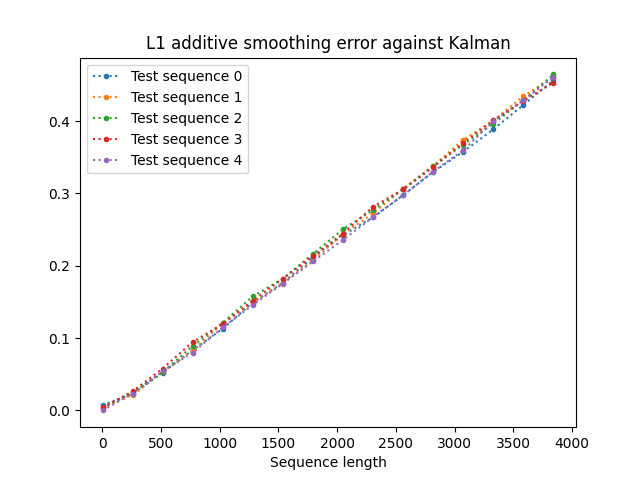
\includegraphics[width=10cm]{additive_smoothing_errors.png}
    \caption{Computation of $\big| \postmod{0:n} h_{0:n} -  \post{0:n}^{\parvec} h_{0:n} \big|$ for growing values of $n$}
\end{figure}

\begin{figure}[h]
    \centering
    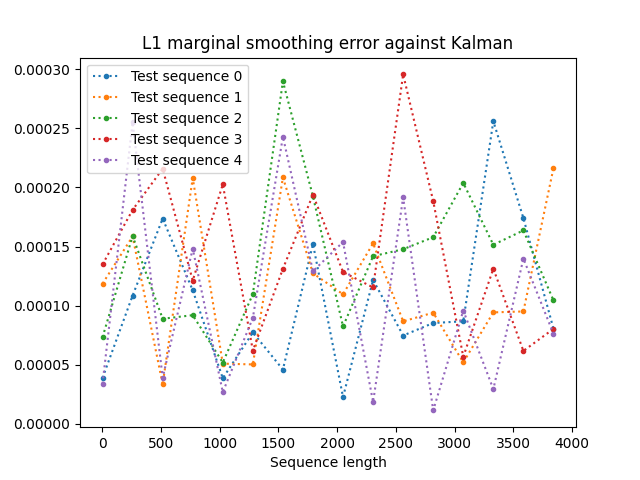
\includegraphics[width=10cm]{marginal_smoothing_errors.png}
    \caption{Computation of $\big| \postmod{0:n} \tilde{h}_{k} -  \post{0:n}^{\parvec} \tilde{h}_{k} \big|$ for different $k$}
\end{figure}

\subsection{Noisy linear ICA}
\textcolor{red}{Comparaisons \`a Kalman/mean field.} 
\subsection{Noisy nonlinear ICA}
\textcolor{red}{Comparaisons \`a l'algo de Hermanni.}

\newpage

%We now want to frame the multi-object tracking challenge as the downstream task of the more general problem of "disentenglement". In general terms and departing from the specific field of computer vision, we view our observations as random variables that arise from a generating process involving hidden/latent random variables. In disentenglement research, these latent variables are assumed to decompose into independent components (which, in the deep learning community, would be refered to as disentangled "representations"). For multi-object tracking, our goal is to infer latent variables whose independent components are "object-centric" representations, ie. each of them separetely describes an individual object. Many works exist that constrain VAEs to provide disentengled latent variables (e.g. via a special form of regularization, see \cite{betavae}) but \cite{unidentifiability} showed that most of them are actually trying to solve an ill-posed problem which is essentially unidentifiable. On the contrary, the Independant Component Analysis (ICA) litterature provides many identifiability results. In brief, in the nonlinear case, identifiability is only guaranteed if signals exhibit some structure (e.g. temporal dependencies), or if the inference is conditioned on an additionally observed process, which was shown in \cite{iVAE} for the specific case of VAEs. More recently, \cite{hermanni2021} proved identifiability when hidden states follow linear but flexible dynamics via regime switching: this is currently the most general setup that is still backed by identifiability proofs. However, in practice, inference is made with strong assumptions on the variational family. For sequential data, this is in contrast to the most recent works on VAEs, like \cite{campbell2021online}, which introduce flexible variational families that factorize according to the original model. We therefore attempt to merge ideas from these works.


In all that follows, we use $\mathsf{X}$ to refer to a set with elements $\mathsf{x} \in \mathsf{X}$ and $\mathsf{X}^p$ the associated product space.  For any set $\mathsf{X}$ we always assume that we can build a $\sigma$-field $\sigma(\mathsf{X})$ and we define $\mathsf{M}_1(\mathsf{X})$ the space of probability measures on $(\mathsf{X},\sigma(\mathsf{X}))$. Let $(\mathsf{\Omega},\mathcal{F},\mathbb{P})$ a probability space, we denote $\mathsf{F(X)}$ the space of all measurable functions from $(\mathsf{\Omega},\mathcal{F})$ to $(\mathsf{X},\sigma(\mathsf{X}))$. We say that "$x$ is a random variable on $\mathsf{X}$ with distribution $p_x$" if $x \in \mathsf{F(X)}$ and $p_x \in \mathsf{M}_1(\mathsf{X})$ satisfies $p_x = \mathbb{P} \circ x^{-1}$.  We define a process $(x_t)_{t \in \mathsf{T}}$ on $\mathsf{X}$ as a collection of random variables indexed by $\mathsf{T}$ and taking values in $\mathsf{X}$. 

When useful, we will sometimes stress on using sans-serif formatting $\mathsf{x}$ for non random objects as opposed to serif formatting $x$ for random objects. However we will often refer to objects and their expressions interchangeably. For example, if $x$ is a random variable in $\mathsf{X}$, we say "the function $f(x) = \ldots $" to refer to a function with input space $\mathsf{F(X)}$ having a given expression, and if $\mathsf{x} \in \mathsf{X}$, we say "the function $f(\mathsf{x}) = \ldots"$ to refer to a function with input space $\mathsf{X}$ having a given expression.We systematically overload the symbol $p$ by using $p(\rmd x)$ to refer to a distribution $p_x$ and interchangeably with its expression $p_x(\mathsf{\rmd x})$. If $x$ and $y$ are random variables on $\mathsf{X}$ and $\mathsf{Y}$, respectively, we write $p(\rmd y|x)$ for the conditional distribution of $y$ given that $x = \mathsf{x}$. In practise, we assume that all distributions $p(\rmd x)$ on $\mathsf{X}$ are dominated w.r.t some reference measure $\mu_x$ on $\sigma(\mathsf{X})$ and admit a probabiltiy density denoted as $p(x)$ (interchangeably with its expression $p(\mathsf{x})$ depending on the context) defined as the Radon-Nikodym derivative $p(x) = \frac{\rmd p_x}{\rmd \mu_x}$. Given all this, we often mix a distribution with its density and say that "$x$ is a random variable with distribution $p(x) = p(\mathsf{x})$" to mean that $x$ is a random variable on $\mathsf{X}$ admitting a density whose expression is $p(\mathsf{x})$. Similarly, we will refer to "$p(x_t|x_{t-1}) = p(x_t|\mathsf{x}_{t-1})$" when a Markovian process $(x_t)_{t \in \mathsf{T}}$ is defined by a Markov kernel which admits a density expressed by $p(x_t|\mathsf{x}_{t-1})$.



\subsection{Nonlinear ICA with flexible dynamics}\label{nonlinear_ica}

In this section, we introduce the setting of nonlinear ICA and define the models that form the basis of our work. Let $(x_t)_{t \geq 1}$ be a process in an $d_\mathsf{X}$-dimensional space $\mathsf{X}$ and for which we assume that:
$$x_t = f(s_t) + \epsilon_t$$

In the ICA setting, $(s_t)_{t \geq 1}$ is a process in $\mathsf{S}^I$ with $\dim(\mathsf{S}) = d_\mathsf{S}$ and $I \in \mathbb{N}^{*}$. In the nonlinear case, $f$ is a nonlinear mapping from $\mathsf{S}^I$ to $\mathsf{X}$ and is usually supposed to be injective. The central assumption is that the components $(s_t^i)_{i \leq I}$ are mutually independant random variables on $\mathsf{S}$.

In a general setting, these variables can follow their own temporal dynamics. Transitions are defined component-wise and can also be conditioned on another (unobserved) process $(u_t)_{t \geq 1}$ on a space $\mathsf{U}^I$ for which each of the $(u_t^i)_{i \leq I}$ is a first order Markov chain in $\mathsf{U}$ with Markov kernel $p(u_t^i|u_{t-1}^i)$ and initial distribution $p(u_1^i)$. Finally, rich models with complex dependencies are allowed by prescribing the transitions in the augmented state space $\mathsf{H} = \mathsf{S}^D$ instead of $\mathsf{S}$, with $D > 1$. Denoting $(h_t)_{t \geq 1}$ the process in the augmented space, each $(h_t^i)_{t \geq 1}$ is a Markov chain in $\mathsf{H}$ conditonally on $(u_t^i)_{t \geq 1}$ with Markov kernel $p(h_t^i|h_{t-1}^i,u_t^i)$ and initial distribution $p(h_1^i|u_1^i)$.

Denote $z_t = (z_t^i)_{i \leq I} \in \mathsf{Z}^I$ the full latent state at time $t$ defined by $z_t^i = (h_t^i, u_t^i)$, where $\mathsf{Z} = \mathsf{H} \times \mathsf{U}$. Each $(z_t^i)_{i \leq I}$ is also a Markov chain in $\mathsf{Z}$ with Markov kernel defined as $p(z_t^i|z_{t-1}^i) = p(h_t^i,u_t^i|h_{t-1}^i, u_{t-1}^i)$ = $p(h_t^i|h_{t-1}^i,u_t^i)p(u_t^i|u_{t-1}^i)$. With all that, $(z_t)_{t \geq 1}$ is a Markov chain in $\mathsf{Z}^I$ with inital distribution $p(z_1)$ and kernel

\begin{equation}\label{kernel_z}
    p(z_t|z_{t-1}) = \prod_{i=1}^I p(z_t^i|z_{t-1}^i)
\end{equation}


Simply put $(z_t)_{z \geq 1}$ is just a special form of autoregressive process with independant components. The full data model is given by the finite dimensional law $p(x_{1:T}, s_{1:T}, u_{1:T})$ which is a marginal of its counterpart in augmented space $p(x_{1:T}, z_{1:T}) = p(x_{1:T} \vert z_{1:T})p(z_{1:T})$. At each time $t$, $x_t$ only depends on $s_t$, and observations $(x_t)_{t \leq T}$ are conditionally independant given $(s_t)_{t \leq T}$, therefore $p(x_{1:T} \vert z_{1:T}) = \prod_{t=1}^T p(x_t|s_t)$. All in all, the full data model writes


\begin{equation}\label{full_model}
    p(x_{1:T}, z_{1:T}) = p(u_1)p(h_1|u_1) p(x_1|s_1) \prod_{t=2}^T p(x_t|s_t) \prod_{i=1}^I p(h_t^i|h_{t-1}^i,u_t^i)p(u_t^i|u_{t-1}^i)
\end{equation} 

\subsection{Variational inference for linear Gaussian HMMs}\label{linear_gauss}
\subsubsection*{Small recap on variational inference}
Given observation vectors $x_{1:T}$, we seek to compute the posterior distributions $p( z_{1:T}|x_{1:T})$. To cope with scenarios where $d_{\mathsf{S}}$ and/or $D$ may be large, we resort to variational inference and want to compute an approximation $q( z_{1:T}|x_{1:T}) \in \mathcal{Q}$ where $\mathcal{Q}$ is a family of distributions that we need to choose. 
We consider an online setup where observations $x_t$ are provided sequentially. From now on we write $p_{1:t}$ for any distribution conditional on $x_{1:t} = \mathsf{x}_{1:t}$. We assume that the best approximation $q_{1:t}^*(z_{1:t}) \in \mathcal{Q}$ (in Kullback-Leibler sense) of $p_{1:t}( z_{1:t})$ can be approached by finding $\argmax\limits_{q \in \mathcal{Q}} \mathcal{L}_t(q)$ where $\mathcal{L}_t(q) = \expect{q(z_{1:t})}{\log\frac{p(z_{1:t}, \mathsf{x}_{1:t})}{q(z_{1:t})}}$. 
Estimates of this optimum are usually available via gradient-based techniques which require assumptions on $\mathcal{Q}$. 
Denoting $\mathcal{P}$ be the family of distributions in which the true posterior $p_{1:t}$ belongs, a sensible choice is to have $\mathcal{Q}$ that closely resembles $\mathcal{P}$ while making optimization tractable. 
\subsubsection*{A simplified fully linear model}
From section \ref{nonlinear_ica}, we start by restricting $\mathcal{P}$ to a much simpler family. We first assume that there is no switching process and that each of the $h_t^i$ follows separate linear Gaussian dynamics defined by parameters $A^i,a^i$ and a Gaussian noise $\eta^i \sim \gaussian{0}{Q^i}$, (the initial distribution is Gaussian with parameters $a_1^i$ and covariance matrix $Q_1^i$). In this case $z_t^i = h_t^i$ and we stick to using $z$ in the following. We also assume that the observation model is time-independant linear Gaussian with parameters $B$ and $b$ and covariance matrix $R$.
Decomposing $z_t^i = \begin{bmatrix}
    s_t^i \\
    S_t^i
    \end{bmatrix}$ 
with each $S_t^i \in \mathsf{S}^{D-1}$, the model is therefore
$$p(z_1^i) \sim \gaussian{a_1^i}{Q_1^i}, \eqsp p(z_1) = \prod_{i=1}^I p(z_1^i)$$
$$p(z_t^i|z_{t-1}^i) \sim \gaussian{A^i z_{t-1}^i + a^i}{Q^i}, \eqsp p(z_t|z_{t-1}) = \prod_{i=1}^I p(z_t^i|z_{t-1}^i)$$
$$p(x_t|z_t) \sim \gaussian{B s_t + b}{R}$$

Since, $p_{1:t}( z_{1:t}) = \frac{p(\mathsf{x}_{1:t},  z_{1:t})}{\int p(\mathsf{x}_{1:t},  z'_{1:t})}$, $p_{1:t}$ is fully specified given parameters $\Theta = \{B, b, R, (A^i, a_1^i, a^i, Q_1^i, Q^i)_{i \leq I}\}$ of the joint model. 
\subsubsection*{A recursion for the ELBO}
The tower property of expectations is such that: 

\begin{equation}
    \mathcal{L}_t(q_{1:t}) = \expect{q_{1:t}( z_{1:t})}{\log \frac{p(x_{1:t},z_{1:t})}{q_{1:t}(z_{1:t})}} = \expect{q_{1:t}( z_t)}{V_t(z_{t})}
\end{equation}

where we have defined $$V_t(z_t) = \expect{q_{1:t}( z_{1:t-1}|z_t)}{\log \frac{p(x_{1:t},z_{1:t})}{q_{1:t}(z_{1:t})}}$$

We denote the forward kernel $p_{(s)}(z_s|z_{s-1}) = p(z_s,x_s|z_{s-1}, x_{s-1}) = p(x_s|z_s)p(z_s|z_{s-1})$ (using the subscript $_{(s)}$ to avoid the confusion $p(z_s,x_s|z_{s-1}) \neq p(z_s|z_{s-1},x_s)$, together with $"s = s:s"$). Note that there is no dependency on $x_{s-1}$ because of HMM structure of our model, this is not true in the general case. Using this notation the numerator in the $\log$ becomes $\prod_{s=1}^t p_{(s)}( z_s|z_{s-1})$. 

In the true model, the distributions $\left\{p_{1:t}(z_{1:t})\right\}_{t \geq 1}$ are the smoothing distributions, which verify the recursion $p_{1:t}(z_{1:t}) = \tilde{p}_{1:t}(z_t|z_{t-1}) p_{1:t-1}(z_{1:t-1})$ where we have defined $$\tilde{p}_{1:t}(z_t|z_{t-1}) = \frac{p_{(t)}(z_{t}|z_{t-1})}{\int p_{(t)}(z_{t}|z_{t-1})p_{1:t-1}(z_{1:t-1})\rmd z_{1:t}}$$

Suppose we choose a variational family where we can define some $\tilde{q}$ that allows the same decomposition $q_{1:t}(z_{1:t}) = \tilde{q}_{1:t}(z_t|z_{t-1}) q_{1:t-1}(z_{1:t-1})$, then we have a recursion for $V_t$, because
\begin{align*}
V_{t+1}(z_{t+1}) &= \expect{q_{1:t}(z_{1:t}|z_{t+1})}{\log \frac{p(x_{1:t+1},z_{1:t+1})}{q_{1:t+1}(z_{1:t+1})}} \\
                   &= \expect{q_{1:t}(z_{1:t}|z_{t+1})}{\log\frac{p_{(t+1)}(z_{t+1}|z_t)\prod_{s=1}^t p_{(s)}(z_s|z_{s-1})}{\tilde{q}_{1:t+1}(z_{t+1}|z_t)\prod_{s=1}^t \tilde{q}_{1:s}(z_s|z_{s-1})}}\\
                   &= \expect{q_{1:t}(z_{1:t}|z_{t+1})}{\log\frac{p_{(t+1)}(z_{t+1}|z_t)}{\tilde{q}_{1:t+1}(z_{t+1}|z_t)} + \log\frac{\prod_{s=1}^t p_{(s)}(z_s|z_{s-1})}{\prod_{s=1}^t \tilde{q}_{1:s}(z_s|z_{s-1})}} \\
                   &= \expect{q_{1:t}( z_t|z_{t+1})}{\expect{q_{1:t}(z_{1:t-1}|z_t,z_{t+1})}{
                           \log\frac{p_{(t+1)}(z_{t+1}|z_t)}{\tilde{q}_{1:t+1}(z_{t+1}|z_t)} + \log\frac{\prod_{s=1}^t p_{(s)}(z_s|z_{s-1})}{\prod_{s=1}^t \tilde{q}_{1:s}(z_s|z_{s-1})}}}
\end{align*}
where the last equality is the tower rule applied once more. 

Suppose that we choose a variational family such that 
\begin{equation}\label{backward_fact}
    q_{1:t}(z_{1:t}) = \vfilt{t}\prod_{s=1}^{t-1} q_{1:s}(z_s|z_{s+1})\eqsp,
\end{equation}
then and $q_{1:t}(z_{1:t-1}|z_t, z_{t+1}) = q_{1:t}(z_{1:t-1}|z_t)$ so

\begin{equation}\label{v_t_recursion}
    V_{t+1}(z_{t+1}) = \expect{\vbackward{t}}{V_t(z_t) + \log\frac{p_{(t+1)}(z_{t+1}|z_t)}{\tilde{q}_{1:t+1}(z_{t+1}|z_t)}}
\end{equation}

with 

\begin{equation}
    \tilde{q}_{1:t+1}(z_{t+1}|z_t) = \frac{\vbackward{t}\vfilt{t+1}}{\vfilt{t}}
\end{equation}

\subsubsection*{A fully tractacle variational approximation}
This recursion is useful provided that we can compute the expectation of the $\log$ term (decomposed as the $\log$ difference) under the backward distribution $\vbackward{t}$. 

In a general HMM, we know that:

\begin{itemize}
    \item Conditionally on $(x_t)_{t \leq T}$, $(z_t)_{t \leq T}$ is a Markov chain backward in time with initial distribution $p_{1:t}(z_t)$, ie. the true smoothing distribution $p_{1:t}(z_{1:t})$ does factorize as in eq. \ref{backward_fact}.
    \item The backward kernel is related to the filtering distribution via: $$p_{1:t}(z_t|z_{t+1}) = \frac{p(z_{t+1}|z_t)p_{1:t}(z_t)}{\int p(z_{t+1}|z_t)p_{1:t}(z_t)\rmd z_t}$$
\end{itemize} 

In the specific case of our more restricted (linear Gaussian) model, we further know, before detailing the computations, that:

\begin{itemize}
    \item The filtering distribution is a Gaussian $p_{1:t}(z_t) \sim \gaussian{\mu_{1:t}}{\Sigma_{1:t}}$
    \item Since $p(z_{t+1}|z_t)$ is a Gaussian where only the mean depends on $z_t$, the numerator in eq. \ref{v_t_recursion} is a Gaussian in $z_t$ and the integral in the denominator is the expected value of that Gaussian distribution. Therefore the backward kernel is also a Gaussian distribution where only the mean depends on $z_{t+1}$. 
\end{itemize} 

With similar reasonings, $\log p_{(t+1)}(z_{t+1}|z_t)$ and $\log \tilde{p}_{1:t+1}(z_{t+1}|z_t)$ are both quadratic forms in $z_t$. This means that if we choose a variational family where this is also true for $\tilde{q}_{1:t+1}(z_{t+1}|z_t)$, then the expectation in the recursion \ref{v_t_recursion} will admit a closed form which is a quadratic form in $z_{t+1}$.
                                                    
One obvious way to choose a variational family that verifies the previous constraints is to define a variational model which mirrors exactly the true model but with different parameters. We start with this option and define the following distributions. We define $\Phi = \{B^\phi, b^\phi, R^\phi, (A^{\phi,i}, a_1^{\phi,i}, a^{\phi,i}, Q_1^{\phi,i}, Q^{\phi,i})_{i \leq I}\}$ the set of all variational parameters, and the following distributions:

$$q(z_1^i) \sim \gaussian{a_1^{\phi,i}}{Q_1^{\phi,i}}, \eqsp q(z_1) = \prod_{i=1}^I q(z_1^i)$$
$$q(z_t^i|z_{t-1}^i) \sim \gaussian{A^{\phi,i} z_{t-1}^i + a^{\phi,i}}{Q^{\phi,i}}, \eqsp q(z_t|z_{t-1}) = \prod_{i=1}^I q(z_t^i|z_{t-1}^i)$$
$$q(x_t|z_t) \sim \gaussian{B^\phi s_t + b^\phi}{R}$$

To facilitate computations, we define the block objects $M = diag(M^1, \ldots, M^I)$ for all relevant parameters. We denote $M^\theta$ the parameters of the true model. We now explicitely derive the closed forms for the expectation of all terms in $\ref{v_t_recursion}$ w.r.t parameters in $\Theta$ and $\Phi$. 

Since the model of our variational approximation is also a linear Gaussian HMM, we can define: 

\begin{itemize}
    \item The variational filtering distribution as a Gaussian $\vfilt{t} \sim \gaussian{\mu_{1:t}^\phi}{\Sigma_{1:t}^\phi}$
    \item The backward variational distribution as a Gaussian $\vbackward{t} \sim \gaussian{\vbackwardmean{t}(z_{t+1})}{\vbackwardcov{t}}$ where $\vbackwardmean{t}$ is linear in $z_{t+1}$ with $\vbackwardmean{t}(z_{t+1}) = \backward{A}_{1:t}^\phi z_{t+1} + \backward{a}_{1:t}^\phi$, where $\backward{A}_{1:t}^\phi$ and $\backward{a}_{1:t}^\phi$ can be entirely expressed in terms of $\mu_{1:t}^\phi, \Sigma_{1:t}^\phi$ and parameters in $\Phi$ (which is detailed below).
\end{itemize} 

We start with the terms from the true model $\log p_{(t+1)}(z_{t+1}|z_t) = \log p(x_{t+1}|z_{t+1}) + \log p(z_{t+1}|z_t)$. The first term on the right hand side is completely measured in $\ref{v_t_recursion}$ at $t+1$ and is therefore integrated later against the backward kernel at $t+2$. We first deal with the second term:

\begin{align}
    \log p(z_{t+1}|z_t) &= -\frac{1}{2}\left(d_\mathsf{Z} \log(2\pi) + \log |Q^\theta|\right) - \frac{1}{2}\left[\quadform{(z_{t+1} - A^\theta z_t - a^\theta)}{\stateprec}\right]
\end{align}

For a random variable $u \sim p(u)$ with $\expect{p(u)}{u} = \mu$ and $\mathbb{V}_{p(u)}[u] = \Sigma$, the following holds for any $\Lambda$:
$$\expect{p(u)}{u^T \Lambda u} = tr(\Lambda \Sigma) + \mu^T \Sigma \mu$$

We denote $u = u(z_t) = A^\theta z_t + a^\theta - z_{t+1}$ and $\Lambda = \stateprec$, and we have

\begin{align*}
    \expect{\vbackward{t}}{u^T \Lambda u} &= \expect{z_t \sim \gaussian{\vbackwardmean{t}}{\vbackwardcov{t}}}{u(z_t)^T \Lambda u(z_t)} \\
    &=  \expect{u \sim \gaussian{A^\theta \vbackwardmean{t} + a^\theta - z_{t+1}}{A^\theta \vbackwardcov{t} {A^\theta}^T}}{u^T \Lambda u}
\end{align*}


which allows the computation of the whole term $\log p(z_{t+1}|z_t)$ against the backward kernel and leads to

\begin{multline*}
    \expect{\vbackward{t}}{\log p(z_{t+1}|z_t)} = -\frac{1}{2}\{d_\mathsf{Z} \log(2\pi) + \log |Q^\theta| + tr(\stateprec A^\theta \vbackwardcov{t} {A^\theta}^T) \\
     + \quadform{(A^\theta \vbackwardmean{t}(z_{t+1}) + a^\theta - z_{t+1})}{\stateprec}\} 
\end{multline*}

Where we can see clearly that it is still a quadratic form in $z_{t+1}$ if $\vbackwardmean{t}(z_{t+1})$ is linear in $z_{t+1}$

To express the parameters $\vbackwardmean{t}$ and $\vbackwardcov{t}$ of the variational backward in terms of parameters in $\Phi$ and $\vfiltmean{t},\vfiltcov{t}$, we just recall that: 

\begin{equation*}
    \vbackward{t} \propto q(z_{t+1}|z_t) \vfilt{t} \propto e^{-\frac{1}{2}\left[\quadform{\left(z_{t+1} - (A^\phi z_t + a^\phi)\right)}{\vstateprec} + \quadform{(z_t - \vfiltmean{t})}{\inv{\vfiltcov{t}}} \right]}
\end{equation*}

Quadratic forms develop into $\quadform{(u-b)}{\Omega} = \quadform{u}{\Omega} - 2b^T \Omega u +b^T \Omega b$ (for $\Omega$ symmetric), so for any $A,b_1,b_2,\Omega_1, \Omega_2$:

\begin{align*}
\quadform{(Au - b_1)}{\Omega_1} + \quadform{(u-b_2)}{\Omega_2} &= \quadform{u}{(A^T\Omega_1 A + \Omega_2)} - 2\left[b_1^T \Omega_1 A + b_2^T \Omega_2 \right]u + \quadform{b_1}{\Omega_1} + \quadform{b_2}{\Omega_2} \\
    &= \quadform{u}{\Omega}
\end{align*}

With $\Omega = (\quadform{A}{\Omega_1}+ \Omega_2)$ and $b = \inv{\Omega}\left(\Omega_2 b_2 + A^T \Omega_1 b_1 \right)$.

This operation is precisely what appears in the argument of the exponential in the previous equation with $A = A^\phi$, $b_1 = z_{t+1} - a^\phi$, $\Omega_1 = \vstateprec$, $b_2 = \vfiltmean{t}$, $\Omega_2 = \inv{\vfiltcov{t}}$, so we can identify the parameters of $\vbackward{t}$ as 

$$\vbackwardcov{t} = \inv{\left(\quadform{{A^\phi}}{\vstateprec} + \inv{\vfiltcov{t}}\right)}$$

$$\vbackwardmean{t} = \left(\quadform{{A^\phi}}{\vstateprec} + \inv{\vfiltcov{t}}\right)\left(\inv{\vfiltcov{t}}\vfiltmean{t} + {A^\phi}^T \vstateprec (z_{t+1} - a^\phi)\right)$$

Therefore we do have the linearity in $z_{t+1}$ with $$\backward{A}_{1:t}^\phi = \left(\quadform{{A^\phi}}{\vstateprec} + \inv{\vfiltcov{t}}\right) {A^\phi}^T \vstateprec$$ and $$\backward{a}_{1:t}^\phi = \left(\quadform{{A^\phi}}{\vstateprec} + \inv{\vfiltcov{t}}\right)\left(\inv{\vfiltcov{t}}\vfiltmean{t} - {A^\phi}^T \vstateprec a^\phi \right)$$


It remains to compute $\expect{\vbackward{t}}{\log \tilde{q}_{1:t+1}(z_{t+1}|z_t)}$ which develops into
\begin{multline*}
    \expect{\vbackward{t}}{\log \tilde{q}_{1:t+1}(z_{t+1}|z_t)}= \expect{\vbackward{t}}{\log \vbackward{t}} + \expect{\vbackward{t}}{\log \vfilt{t+1}} \\ 
    - \expect{\vbackward{t}}{\log \vfilt{t}}
\end{multline*}

The second term is only integrated at $t+2$ but cancels out with the third term (from $t+2$) ie. the $\log$ of the filtering distributions form a telecoping series. Therefore we only need to integrate the third term at the $t=2$ and evaluate the second one at $t=T$. The first term is the expectation of the log-backward under the backward, ie. the expectation of the log of a Gaussian under iself which yields $-\frac{1}{2}\left(d_{\mathsf{Z}}(\log 2\pi + 1) + \log |\vbackwardcov{t}|\right)$

For the observation model at $t+2$ we have

\begin{multline*}
\expect{q_{1:t+1}(z_{t+1}|z_{t+2})}{\log p(x_{t+1}|z_{t+1})} = -\frac{1}{2}\{d_{\mathsf{X}}\log 2\pi + \log |R^\theta| + tr\left(\inv{R^\theta} B^\theta\vbackwardcov{t+1}{B^\theta}^T\right) \\ + \quadform{(B^\theta\vbackwardmean{t+1} + b^\theta - x_{t+1})}{\inv{R^\theta}}\}
\end{multline*} 


\subsection{Extensions}

In the linear Gaussian case, we were able to derive all results in closed-form without any approximation. For this model, optimal estimation of the smoothing distribution and the model parameters is already avaible via the Kalman smoothing recursions coupled with EM optimization or recursive likelihood maximization. 

Provided that $(z_t,x_t)_{t \geq 1}$ is still a HMM, the backward factorization of the joint smoothing distribution always exists for the true model, and is therefore a theoretically motivated choice for constraining the variational family as in \ref{backward_fact}. Given this factorization, the recursion \ref{v_t_recursion} is always true. Therefore, for more general cases the variational family may be more conviently defined directly via the backward kernel. 

In general, if the true model is not assumed to be linear Gaussian, none of the posterior distributions (joint and marginal smoothing or filtering) are Gaussian, and therefore the backward kernels (related to the filtering distributions) are not Gaussian either. Even if we prescribe Gaussianity for the variational terms, the log terms from the true model are not easily integrated against the variational backward because they are not quadratic forms anymore. 

As explained in introduction, identifiabilty results in ICA only exist for models with linear dynamics (though with the possibility of regimes as in section \ref{nonlinear_ica}) so we do not consider nonlinear transitions for the hidden state. Yet, nonlinearity in the observation model alone still breaks the gaussianity of the posteriors. In this case, particle methods can be used to build discretely-supported unbiased and online approximators of the filtering distribution $p_{1:t}(z_t)$. However they suffer from the curse of dimensionality because the number of particle grows linearly with the $d_{\mathsf{Z}}$, which makes them unsuitable to estimate representions that are expressive enough for complex sources (e.g. visual descriptors of individual objects in computer vision, properties of individual speakers in audio, etc). What's more, even if $d_{\mathsf{Z}}$ is small enough, the support of the joint $p_{1:t}(z_{1:t})$ is increasing in $t$, and therefore particle methods can typically only provide estimators of expectations $\expect{p_{1:t}(z_{1:t})}{h(z_{1:t})}$. In this context, it therefore makes sense to stick to variational inference, which is the only tractable tool to provide an approximation of the full joint smoothing distribution. 

In the VAE litterature, powerful variational families (e.g. normalizing flows) are now frequently considered to obtain expressive posteriors. However, we show in this section that many terms in section \ref{linear_gauss} become intractble even when sticking to Gaussian parameterization, and we provide an overview of the different tools which can be used to approximate the latter. 

\subsubsection*{Replacing the Kalman update with a learnt filtering recursion}
\dots

\subsubsection*{Nonlinear observation model}

We assume a similar transition model $p(z_t|z_{t-1})$ for the hidden states, but observations are nonlinear transformations of the components under Gaussian noise, ie. $$p(x_t|z_t) = p(x_t|s_t) \sim \gaussian{f_\theta(s_t)}{R^\theta}$$. 

As stated above, in this case, $p_{1:t}(z_t|z_{t+1})$ is not Gaussian anymore, however we approximate it with a Gaussian variational backward $\vbackward{t} \sim \gaussian{\vbackwardmean{t}(z_{t+1})}{\vbackwardcov{t}}$ and define the variational joint smoothing distribution via the backward factorization given by equation \ref{backward_fact}. If we specify that $\vbackwardmean{t}(z_{t+1})$ is linear in $z_{t+1}$, then all quantities in the previous section except from the expectation of the observation model are tractable as before. For this latter term, at $t+2$, 

\begin{multline*}
\expect{q_{1:t+1}(z_{t+1}|z_{t+2})}{\log p(x_{t+1}|z_{t+1})} = -\frac{1}{2}\{d_{\mathsf{X}}\log 2\pi + \log |R^\theta| \\
    + \expect{z_{t+1} \sim \gaussian{\vbackwardmean{t+1}}{\vbackwardcov{t+1}}}{\quadform{(f_\theta(z_{t+1}) - x_{t+1})}{\inv{R^\theta}}}\} \\
\end{multline*}

and the expectation that remains admits no closed-form. From \cite{johnson}, the following approximation may be a suitable alternative (where we write the equation at $t$ for readability)

\begin{equation}
    \expect{\vbackward{t}}{\log p(x_t|z_t)} \propto \eqsp \quadform{[z_{t+1} - v(x_t)]}{W(x_t)}
\end{equation}

where 


\appendix
\section{Proof of Proposition~\ref{prop:bias}}
\label{sec:proof}
Following \cite{gloaguen2019pseudo}, write 
$$
\postmod{0:n} h_n - \post{0:n}^\theta h_n = \sum_{k = 0}^{n - 1} \left( \postmod{0:n} \addf[n]{k} - \post{0:n}^\theta \addf[n]{k} \right), 
$$
where, for each $k \in \intvect{0}{n - 1}$, 
\begin{equation} \label{eq:def:addf}
\addf[n]{k} : (\mathbb{R}^d)^{n+1} \ni x_{0:n} \mapsto \addf{k}(x_k, x_{k + 1}) 
\end{equation}
denote the extension of $\addf{k}$ to $(\mathbb{R}^d)^{n+1}$. Define, for each $n \in \nset$ and $m \in \intvect{0}{n}$, the kernel 
\begin{equation} \label{eq:def:uk:products}
    \uk{m, n}^\theta(x_{0:m}', \rmd x_{0:n + 1}) \eqdef \delta_{x_{0:m}'}(\rmd x_{0:m}) \prod_{\ell = m}^n \uk{\ell,\theta}(x_\ell, \rmd x_{\ell + 1}) 
\end{equation}
on $(\mathbb{R}^d)^{m+1} \times \mathcal{B}((\mathbb{R}^d)^{n + 1})$, with the convention $\uk{n, n - 1}^\theta = \operatorname{id}$.  This yields the following decomposition:
\begin{multline*}
\postmod{0:n} \addf[n]{k} - \post{0:n}^\theta \addf[n]{k} = 
\sum_{m = 1}^n \left( \frac{\postmod{0:m} \uk{m, n - 1}^\theta \addf[n]{k}}{\postmod{0:m} \uk{m, n - 1}^\theta \1_{}} - \frac{\postmod{0:m - 1} \uk{m - 1, n - 1}^\theta \addf[n]{k}}{\postmod{0:m - 1} \uk{m - 1, n - 1}^\theta \1_{}} \right) \\ + \frac{\postmod{0} \uk{0, n - 1}^\theta \addf[n]{k}}{\postmod{0} \uk{0, n - 1}^\theta \1_{}} - \frac{\chi_\theta \md{0;\parvec}\uk{0, n - 1}^\theta \addf[n]{k}}{\chi_\theta\md{0;\parvec}\uk{0, n - 1}^\theta \1_{}},
\end{multline*}
where $\postmod{0} = \postmod{0:0}$, and since $\chi_\theta \md{0;\parvec} \uk{0, n - 1}^\theta \addf[n]{k}/\chi_\theta\md{0;\parvec}\uk{0, n - 1}^\theta \1_{} = \post{0:n}^\theta \addf[n]{k}$.
%For each $m \in \nset$, define the  backward Markov kernel 
%\begin{equation} \label{eq:def:backward:kernel}
%    \bkw{m}^\parvec(x_{m + 1}, \rmd x_m) \eqdef \frac{\post{m}^\parvec(\rmd x_m) \, \ud{m,\parvec}(x_m, x_{m + 1})}{\post{m}^\parvec[\ud{m,\parvec}(\cdot, x_{m + 1})]} = \frac{\post{m}^\parvec(\rmd x_m) \, \hd{m+1;\parvec}(x_{m}, x_{m+1})}{\post{m}^\parvec[\hd{m+1;\parvec}(\cdot, x_{m+1})]}
%\end{equation}
%on $\mathbb{R}^d \times \mathcal{B}(\mathbb{R}^d)$. In addition, for each $n>0$, define on $\mathbb{R}^d \times \mathcal{B}((\mathbb{R}^d)^n)$ the following Markov kernel  : 
%\begin{equation} \label{eq:def:tstat}
%\tstat{n}^\parvec(x_n, \rmd x_{0:n - 1}) \eqdef \prod_{m = 0}^{n - 1} \bkw{m}^\parvec(x_{m + 1}, \rmd x_m)
%\end{equation}
%%on $\Xset_n \times \Xfd^{n - 1}$ denote the joint law of the backward Markov chain induced by the kernels \eqref{eq:def:backward:kernel} when initialised at $x_n \in \Xset_n$.   
%%In the following, the notation $\parvec$ may be dropped when there is no confusion. 
%Define similarly, 
%$$
%\bkw{m}^\varphi(x_{m + 1}, \rmd x_m) = q_{\varphi,m}(x_{m+1},x_m)\mu(\rmd x_m)
%$$
%on $\mathbb{R}^d \times \mathcal{B}(\mathbb{R}^d)$. 
In addition, define for each $n \in \nsetpos$, the Markov kernel  
$$
\tstat{n}^\varphi(x_n, \rmd x_{0:n - 1}) = \prod_{m = 0}^{n - 1} Q_{\varphi,m}(x_{m + 1}, \rmd x_m)
$$ 
on $\mathbb{R}^d \times \mathcal{B}((\mathbb{R}^d)^n)$. % In the following, the notation $\parvec$ may be dropped when there is no confusion. 
%\begin{itemize} 
%\item[(i)]
%For all $n \in \nset$ and $h \in \bmf{\Xfd_n \tensprod \Xfd_{n + 1}}$, 
%\begin{equation} \label{eq:reversibility}
%\iint \post{n}^\parvec(\rmd x_n) \, \uk{n,\parvec}(x_n, \rmd x_{n + 1}) \, h(x_n, x_{n + 1}) = \iint \post{n}^\parvec \uk{n,\parvec}(\rmd x_{n + 1}) \, \bkw{n}^\parvec(x_{n + 1}, \rmd x_n) \, h(x_n, x_{n + 1}). 
%\end{equation}
%\item[(ii)]
%For all $n \in \nsetpos$ and $h \in \bmf{\Xfd^n}$, 
%$
%\post{0:n}^\parvec h = \post{n}^\parvec \tstat{n}^\parvec h. 
%$
%\end{itemize}
%\begin{proof}
    For each $n \in \nset$, define  $\retrokmod_{0, n}(x_0', \rmd x_{0:n}) \eqdef \delta_{x_0'}(\rmd x_0) \,  \prod_{\ell = 0}^{n - 1} \uk{\ell,\theta}(x_\ell, \rmd x_{\ell + 1})$ and for $m \in \intvect{1}{n}$, 
\begin{equation} \label{eq:def:retrokmod}
    \retrokmod_{m, n}(x_m', \rmd x_{0:n}) \eqdef \delta_{x_m'}(\rmd x_m) \, \tstatmod{m}(x_m, \rmd x_{0:m - 1}) \prod_{\ell = m}^{n - 1} \uk{\ell,\theta}(x_\ell, \rmd x_{\ell + 1}), 
\end{equation}
on  $\mathbb{R}^d \times \mathcal{B}((\mathbb{R}^d)^{n+1})$. 
As for all $m \in \intvect{0}{n}$ and measurable function $h$, 
%\begin{equation} \label{eq:retro:prospective:id}
 $\postmod{0:m} \uk{m, n - 1}^\theta h = \postmod{m} \retrokmod_{m, n} h$,
%\end{equation}
%In order to bound each term of this decomposition, write, using Lemma~\ref{lem:retro:prospective:id},  
$$
\frac{\postmod{0:m} \uk{m, n - 1}^\theta \addf[n]{k}}{\postmod{0:m} \uk{m, n - 1}^\theta \1_{}} - \frac{\postmod{0:m - 1} \uk{m - 1, n - 1}^\theta \addf[n]{k}}{\postmod{0:m - 1} \uk{m - 1, n - 1}^\theta \1_{}} 
= \frac{\postmod{m} \retrokmod_{m, n} \addf[n]{k}}{\postmod{m} \retrokmod_{m, n} \1_{}} - \frac{\postmod{m - 1} \retrokmod_{m - 1, n} \addf[n]{k}}{\postmod{m - 1} \retrokmod_{m - 1, n} \1_{}}. 
$$
Therefore,
\begin{multline}
\label{eq:error:decomp}
\postmod{0:n} \addf[n]{k} - \post{0:n}^\theta \addf[n]{k} = 
\sum_{m = 1}^n \left( \frac{\postmod{m} \retrokmod_{m, n} \addf[n]{k}}{\postmod{m} \retrokmod_{m, n} \1_{}} - \frac{\postmod{m - 1} \retrokmod_{m - 1, n} \addf[n]{k}}{\postmod{m - 1} \retrokmod_{m - 1, n} \1_{}} \right) \\ + \frac{\postmod{0} \uk{0, n - 1}^\theta \addf[n]{k}}{\postmod{0} \uk{0, n - 1}^\theta \1_{}} - \frac{\chi_\theta \md{0;\parvec}\uk{0, n - 1}^\theta \addf[n]{k}}{\chi_\theta\md{0;\parvec}\uk{0, n - 1}^\theta \1_{}}.
\end{multline}

\paragraph{Error term at time $m=0$ in \eqref{eq:error:decomp}. }Consider the following decomposition of the first term:
\begin{align*}
\frac{\postmod{0} \uk{0, n - 1}^\theta \addf[n]{k}}{\postmod{0} \uk{0, n - 1}^\theta \1_{}} - \frac{\chi_\theta \md{0;\parvec}\uk{0, n - 1}^\theta \addf[n]{k}}{\chi_\theta\md{0;\parvec}\uk{0, n - 1}^\theta \1_{}} &= \frac{\postmod{0} \uk{0, n - 1}^\theta \addf[n]{k}}{\postmod{0} \uk{0, n - 1}^\theta \1_{}} - \frac{\phi^\theta_0\uk{0, n - 1}^\theta \addf[n]{k}}{\phi^\theta_0\uk{0, n - 1}^\theta \1_{}}\eqsp,\\
& = \frac{\postmod{0} \uk{0, n - 1}^\theta \addf[n]{k}-\phi^\theta_0\uk{0, n - 1}^\theta \addf[n]{k}}{\postmod{0} \uk{0, n - 1}^\theta \1_{}} \\
&\hspace{2cm}+  \frac{\phi^\theta_0\uk{0, n - 1}^\theta \addf[n]{k}}{\phi^\theta_0\uk{0, n - 1}^\theta \1_{}}\frac{\phi^\theta_0\uk{0, n - 1}^\theta \1_{} - \postmod{0} \uk{0, n - 1}^\theta \1_{}}{\postmod{0} \uk{0, n - 1}^\theta \1_{}} \eqsp,
\end{align*}
where $\phi^\theta_0$ the filtering distribution at time $0$, i.e the law defined as  $\phi^\theta_0h= \chi_\theta \md{0;\parvec}h/\chi_\theta \md{0;\parvec}$. Then, by H\ref{assum:bias:bound},
$$
\left|\frac{\postmod{0} \uk{0, n - 1}^\theta \addf[n]{k}}{\postmod{0} \uk{0, n - 1}^\theta \1_{}} - \frac{\phi^\theta_0\uk{0, n - 1}^\theta \addf[n]{k}}{\phi^\theta_0\uk{0, n - 1}^\theta \1_{}}\right|\leqslant 2c_0(\theta,\varphi)\frac{\| \uk{0, n - 1}^\theta \1_{}\|_\infty\|\addf[n]{k}\|_\infty}{\postmod{0} \uk{0, n - 1}^\theta \1_{}}\eqsp.
$$
By H\ref{assum:strong:mixing}, for all $x_0\in \mathbb{R}^d$,
$$
\uk{0, n - 1}^\theta \1_{}(x_0) = \int  \ud{0,\parvec}(x_0, x_{1})\mu(\rmd x_1)\uk{1, n - 1}^\theta \1_{}(x_1)\leqslant \sigma_+  \int \mu(\rmd x_1)\uk{1, n - 1}^\theta \1_{}(x_1)
$$
and 
$$
\postmod{0} \uk{0, n - 1}^\theta \1 = \int \postmod{0} (\rmd x_0)\ud{0,\parvec}(x_0, x_{1})\mu(\rmd x_1)\uk{1, n - 1}^\theta \1_{}(x_1)\geqslant \sigma_-  \int \mu(\rmd x_1)\uk{1, n - 1}^\theta \1_{}(x_1)\eqsp,
$$
which yields
$$
\left|\frac{\postmod{0} \uk{0, n - 1}^\theta \addf[n]{k}}{\postmod{0} \uk{0, n - 1}^\theta \1_{}} - \frac{\phi^\theta_0\uk{0, n - 1}^\theta \addf[n]{k}}{\phi^\theta_0\uk{0, n - 1}^\theta \1_{}}\right|\leqslant 2c_0(\theta,\varphi)\frac{\sigma_+}{\sigma_-}\|\addf[n]{k}\|_\infty\eqsp.
$$

\paragraph{Error term at time $m>0$ in \eqref{eq:error:decomp}. } Define the kernel  
\begin{equation} \label{eq:def:retrokmod:joint}
    \tilde{\mathcal{L}}^{\varphi,\theta}_{m, n}(x'_{m-1},x_m', \rmd x_{0:n}) \eqdef \delta_{x'_{m-1}}(\rmd x_{m-1})\delta_{x_m'}(\rmd x_m) \, \tstatmod{m-1}(x_{m-1}, \rmd x_{0:m - 2}) \prod_{\ell = m}^{n - 1} \uk{\ell,\theta}(x_\ell, \rmd x_{\ell + 1}), 
\end{equation}
on  $(\mathbb{R}^d)^2 \times \mathcal{B}((\mathbb{R}^d)^{n+1})$.  Then, write
$$
 \frac{\postmod{m} \retrokmod_{m, n} \addf[n]{k}}{\postmod{m} \retrokmod_{m, n} \1_{}} - \frac{\postmod{m - 1} \retrokmod_{m - 1, n} \addf[n]{k}}{\postmod{m - 1} \retrokmod_{m - 1, n} \1_{}}  = \frac{\postmod{m} Q_{\varphi,m-1} \tilde{\mathcal{L}}^{\varphi,\theta}_{m, n} \addf[n]{k}}{\postmod{m} \retrokmod_{m, n} \1_{}} - \frac{\postmod{m - 1} \uk{m-1,\theta} \tilde{\mathcal{L}}^{\varphi,\theta}_{m, n} \addf[n]{k}}{\postmod{m - 1} \retrokmod_{m - 1, n} \1_{}} \eqsp.
$$
Let $x_{m-1}^*$ and $x_m^*$ be arbitrary elements in $\mathbb{R}^d$ and define the kernel
$$
\mathcal{L}^{*,\varphi,\theta}_{m, n}h(x_{m-1},x_m) = \frac{\tilde{\mathcal{L}}^{\varphi,\theta}_{m, n}h(x_{m-1},x_m) }{\tilde{\mathcal{L}}^{\varphi,\theta}_{m, n}\1(x_{m-1},x_m)} - \frac{\tilde{\mathcal{L}}^{\varphi,\theta}_{m, n}h(x^*_{m-1},x^*_m) }{\tilde{\mathcal{L}}^{\varphi,\theta}_{m, n}\1(x^*_{m-1},x^*_m)} = \frac{\tilde{\mathcal{L}}^{\varphi,\theta}_{m, n}h(x_{m-1},x_m) }{\uk{m, n - 1}^\theta\1(x_m)} - \frac{\tilde{\mathcal{L}}^{\varphi,\theta}_{m, n}h(x^*_{m-1},x^*_m) }{\uk{m, n - 1}^\theta\1(x^*_m)}\eqsp,
$$
and define the normalized measure $\tilde\phi^\varphi_mh$ by $\postmod{m - 1} \uk{m-1,\theta}h/\postmod{m - 1} \uk{m-1,\theta}\1$, so that
\begin{align*}
 \frac{\postmod{m} \retrokmod_{m, n} \addf[n]{k}}{\postmod{m} \retrokmod_{m, n} \1_{}} &- \frac{\postmod{m - 1} \retrokmod_{m - 1, n} \addf[n]{k}}{\postmod{m - 1} \retrokmod_{m - 1, n} \1_{}}  \\
&= \frac{\postmod{m} Q_{\varphi,m-1} \left\{\mathcal{L}^{*,\varphi,\theta}_{m, n} \addf[n]{k}\tilde{\mathcal{L}}^{\varphi,\theta}_{m, n} \1\right\}}{\postmod{m} \retrokmod_{m, n} \1_{}} - \frac{\postmod{m - 1} \uk{m-1,\theta} \left\{\mathcal{L}^{*,\varphi,\theta}_{m, n} \addf[n]{k}\tilde{\mathcal{L}}^{\varphi,\theta}_{m, n} \1\right\}}{\postmod{m - 1} \retrokmod_{m - 1, n} \1_{}} \\ 
&=  \frac{\postmod{m} Q_{\varphi,m-1} \left\{\mathcal{L}^{*,\varphi,\theta}_{m, n} \addf[n]{k}\tilde{\mathcal{L}}^{\varphi,\theta}_{m, n} \1\right\}}{\postmod{m} \retrokmod_{m, n} \1_{}} - \frac{\tilde\phi^\varphi_m\left\{\mathcal{L}^{*,\varphi,\theta}_{m, n} \addf[n]{k}\tilde{\mathcal{L}}^{\varphi,\theta}_{m, n} \1\right\}}{\tilde\phi^\varphi_m\tilde{\mathcal{L}}^{\varphi,\theta}_{m, n}\1_{}} \\ \\
&= \frac{\postmod{m} Q_{\varphi,m-1} \left\{\mathcal{L}^{*,\varphi,\theta}_{m, n} \addf[n]{k}\tilde{\mathcal{L}}^{\varphi,\theta}_{m, n} \1\right\} - \tilde\phi^\varphi_m \left\{\mathcal{L}^{*,\varphi,\theta}_{m, n} \addf[n]{k}\tilde{\mathcal{L}}^{\varphi,\theta}_{m, n} \1\right\}}{\tilde\phi^\varphi_m\tilde{\mathcal{L}}^{\varphi,\theta}_{m, n}\1_{}} \\
&\hspace{2.5cm}+  \frac{\postmod{m} Q_{\varphi,m-1}\left\{\mathcal{L}^{*,\varphi,\theta}_{m, n} \addf[n]{k}\tilde{\mathcal{L}}^{\varphi,\theta}_{m, n} \1\right\}}{\postmod{m} \retrokmod_{m, n} \1_{}}\left(\frac{\tilde\phi^\varphi_m\tilde{\mathcal{L}}^{\varphi,\theta}_{m, n}\1-\postmod{m} \retrokmod_{m, n} \1_{}}{\tilde\phi^\varphi_m\tilde{\mathcal{L}}^{\varphi,\theta}_{m, n}\1_{}}\right)\eqsp.
\end{align*}
Then, using that
$$
\left|\frac{\postmod{m} Q_{\varphi,m-1} \left\{\mathcal{L}^{*,\varphi,\theta}_{m, n} \addf[n]{k}\tilde{\mathcal{L}}^{\varphi,\theta}_{m, n} \1\right\}}{\postmod{m} \retrokmod_{m, n} \1_{}}\right|\leqslant \left\|\mathcal{L}^{*,\varphi,\theta}_{m, n} \addf[n]{k}\right\|_\infty\eqsp,
$$
and by H\ref{assum:bias:bound},
\begin{align*}
\left|\frac{\tilde\phi^\varphi_m\tilde{\mathcal{L}}^{\varphi,\theta}_{m, n} \1_{}-\postmod{m} \retrokmod_{m, n} \1_{}}{\tilde\phi^\varphi_m\tilde{\mathcal{L}}^{\varphi,\theta}_{m, n} \1_{}}\right|&\leqslant c_m(\theta,\varphi)\frac{\left\|\tilde{\mathcal{L}}^{\varphi,\theta}_{m, n} \1\right\|_\infty}{\tilde\phi^\varphi_m\tilde{\mathcal{L}}^{\varphi,\theta}_{m, n}\1_{}}\eqsp,\\
\left|\frac{\postmod{m} Q_{\varphi,m-1} \left\{\mathcal{L}^{*,\varphi,\theta}_{m, n} \addf[n]{k}\tilde{\mathcal{L}}^{\varphi,\theta}_{m, n} \1\right\} - \tilde\phi^\varphi_m\left\{\mathcal{L}^{*,\varphi,\theta}_{m, n} \addf[n]{k}\tilde{\mathcal{L}}^{\varphi,\theta}_{m, n} \1\right\}}{\tilde\phi^\varphi_m\tilde{\mathcal{L}}^{\varphi,\theta}_{m, n} \1_{}}\right| &\leqslant c_m(\theta,\varphi)\frac{\left\|\mathcal{L}^{*,\varphi,\theta}_{m, n} \addf[n]{k}\right\|_\infty\left\|\tilde{\mathcal{L}}^{\varphi,\theta}_{m, n} \1\right\|_\infty}{\tilde\phi^\varphi_m\tilde{\mathcal{L}}^{\varphi,\theta}_{m, n}\1_{}}\eqsp,
\end{align*}
yields
$$
\left| \frac{\postmod{m} \retrokmod_{m, n} \addf[n]{k}}{\postmod{m} \retrokmod_{m, n} \1_{}} - \frac{\postmod{m - 1} \retrokmod_{m - 1, n} \addf[n]{k}}{\postmod{m - 1} \retrokmod_{m - 1, n} \1_{}} \right|\leqslant 2c_m(\theta,\varphi)\frac{\left\|\mathcal{L}^{*,\varphi,\theta}_{m, n} \addf[n]{k}\right\|_\infty\left\|\tilde{\mathcal{L}}^{\varphi,\theta}_{m, n} \1\right\|_\infty}{\tilde\phi^\varphi_m\tilde{\mathcal{L}}^{\varphi,\theta}_{m, n}\1_{}}\eqsp.
$$
Note also that by H\ref{assum:strong:mixing},
$$
\tilde\phi^\varphi_m\tilde{\mathcal{L}}^{\varphi,\theta}_{m, n}\1_{} \geqslant \sigma_-^2 \mu  \uk{m+1, n-1}^\theta\1\eqsp,
$$ 
and for all $x,x'\in\mathbb{R}^d$,
$$
\tilde{\mathcal{L}}^{\varphi,\theta}_{m, n} \1(x,x')\leqslant  \sigma_+\mu  \uk{m+1, n-1}^\theta\1\eqsp.
$$
Therefore,

$$
\left| \frac{\postmod{m} \retrokmod_{m, n} \addf[n]{k}}{\postmod{m} \retrokmod_{m, n} \1_{}} - \frac{\postmod{m - 1} \retrokmod_{m - 1, n} \addf[n]{k}}{\postmod{m - 1} \retrokmod_{m - 1, n} \1_{}} \right|\leqslant 2\frac{\sigma_+}{\sigma_-^2}c_m(\theta,\varphi) \left\|\mathcal{L}^{*,\varphi,\theta}_{m, n} \addf[n]{k}\right\|_\infty\eqsp.
$$
The proof is completed using Lemma~\ref{lem:geo:bound}.



%\paragraph{Error term at time $m> k+1$ in \eqref{eq:error:decomp}. } Write
%$$
% \frac{\postmod{m} \retrokmod_{m, n} \addf[n]{k}}{\postmod{m} \retrokmod_{m, n} \1_{}} - \frac{\postmod{m - 1} \retrokmod_{m - 1, n} \addf[n]{k}}{\postmod{m - 1} \retrokmod_{m - 1, n} \1_{}}  = 
%$$

%\clearpage
%\newpage

%Now, for all $m \in \intvect{1}{n}$, pick an arbitrary element $\xarb_m \in \Xset_m$ and define the kernel 
%\begin{equation} \label{eq:def:norm:objective:func}
%\retrokmodnorm_{m, n} h(x_m) \eqdef \frac{\retrokmod_{m, n} h(x_m)}{\retrokmod_{m, n} \1_{\Xset^n}(x_m)} - \frac{\retrokmod_{m, n} h (\xarb_m)}{\retrokmod_{m, n} \1_{\Xset^n} (\xarb_m)}, \quad x_m \in \Xset_m, \quad h \in \bmf{\Xfd^n},
%\end{equation}
%We may express the quantity of interest as 
%\begin{multline*}
%\postmod{0:n} \addf[n]{k} - \post{0:n} \addf[n]{k} = \frac{\postmod{0} \uk{0, n - 1}^\theta \addf[n]{k}}{\postmod{0} \uk{0, n - 1}^\theta \1_{\Xset^n}} - \frac{\chi \uk{0, n - 1}^\theta \addf[n]{k}}{\chi\uk{0, n - 1}^\theta \1_{\Xset^n}} + \sum_{m = 1}^k \left( \noshift_{m, n} \retrokmodnorm_{m, n} \addf[n]{k} - \shiftbwd_{m, n}  \retrokmodnorm_{m, n} \addf[n]{k} \right) \\ 
%+ \frac{\postmod{k + 1} \retrokmod_{k + 1, n} \addf[n]{k}}{\postmod{k + 1} \retrokmod_{k + 1, n} \1_{\Xset^n}} - \frac{\postmod{k} \retrokmod_{k, n} \addf[n]{k}}{\postmod{k} \retrokmod_{k, n} \1_{\Xset^n}} + \sum_{m = k + 1}^{n - 1} \left( \shiftfwd_{m, n} \retrokmodnorm_{m, n} \addf[n]{k} - \noshift_{m, n} \retrokmodnorm_{m, n} \addf[n]{k} \right),
%\end{multline*}
%where, for $h \in \bmf{\Xfd_m}$, 
%\begin{align}
%\noshift_{m, n} h &\eqdef \frac{\postmod{m} (h \times \retrokmod_{m, n} \1_{\Xset^n})}{\postmod{m} \retrokmod_{m, n} \1_{\Xset^n}}, \nonumber \\
%\shiftfwd_{m, n} h &\eqdef \frac{\postmod{m} (h \times \ukmod{m} \retrokmod_{m + 1, n} \1_{\Xset^n})}{\postmod{m} \ukmod{m} \retrokmod_{m + 1, n} \1_{\Xset^n}}, \nonumber \\
%\shiftbwd_{m, n} h &\eqdef \frac{\postmod{m - 1} \uk{m - 1}(h \times \retrokmod_{m, n} \1_{\Xset^n})}{\postmod{m - 1} \retrokmod_{m - 1, n} \1_{\Xset^n}}.  \nonumber 
%\end{align}
%Now, applying Lemmas~\ref{lem:geo:bound} and \ref{lem:diff:bound} to the previous decomposition yields
%$$
%\left| \postmod{0:n} \addf[n]{k} - \post{0:n}^\theta \addf[n]{k} \right| \leq 2 c(\theta,\varphi) \frac{\udup }{\udlow^2} \sum_{k = 0}^{n - 1} \| \addf{k} \|_\infty \left( \sum_{m = 1}^{n - 1} \rho^{|k - m| - 1} + 1 \right),
%$$
%which concludes the proof. 

%
%\medskip
%\medskip
%
%
%
%\begin{lemma} \label{lem:retro:prospective:id}
%For all $m \in \intvect{0}{n}$ and $h \in \bmf{\Xfd^n}$, 
%\begin{equation} \label{eq:retro:prospective:id}
%\postmod{0:m} \uk{m, n - 1} h = \postmod{m} \retrokmod_{m, n} h.  
%\end{equation}
%\end{lemma}



%\begin{lemma} \label{lemma:three:identities}
%Let $n \in \nset$ and $m \in \intvect{1}{n}$. Then the following holds true for all $k \in \intvect{0}{n - 1}$. 
%\begin{itemize}
%\item[(i)]  
%$
%\displaystyle \noshift_{m, n} \left( \frac{\retrokmod_{m, n} \addf[n]{k}}{\retrokmod_{m, n} \1_{\Xset^n}} \right) = \frac{\postmod{m} \retrokmod_{m, n} \addf[n]{k}}{\postmod{m} \retrokmod_{m, n} \1_{\Xset^n}}$ \quad for $m \in \intvect{1}{n}$, 
%\item[(ii)]  
%$
%\displaystyle \shiftfwd_{m, n} \left( \frac{\retrokmod_{m, n} \addf[n]{k}}{\retrokmod_{m, n} \1_{\Xset^n}} \right) = \frac{\postmod{m + 1} \retrokmod_{m + 1, n} \addf[n]{k}}{\postmod{m + 1} \retrokmod_{m + 1, n} \1_{\Xset^n}}
%$ \quad for $m \in \intvect{k + 1}{n}$, and 
%\item[(iii)] 
%$
%\displaystyle \shiftbwd_{m, n} \left( \frac{\retrokmod_{m, n} \addf[n]{k}}{\retrokmod_{m, n} \1_{\Xset^n}} \right) = \frac{\postmod{m - 1} \retrokmod_{m - 1, n} \addf[n]{k}}{\postmod{m - 1} \retrokmod_{m - 1, n} \1_{\Xset^n}}
%$ \quad for all $m \in \intvect{1}{k}$. 
%\end{itemize}
%\end{lemma}
%
%\begin{proof}
%The identity (i) follows straightforwardly by the definition of $\noshift_{m, n}$. We hence turn to (ii), which is established by first noting that for all $m \in \intvect{k + 1}{n}$, 
%$$
%\frac{\retrokmod_{m, n} \addf[n]{k}}{\retrokmod_{m, n} \1_{\Xset^n}} 
%= \bkmod[\postmod{m - 1}]{m - 1} \cdots \bkmod[\postmod{k + 1}]{k + 1} (\bkmod[\postmod{k}]{k} \addf{k}).  
%$$
%Now, 
%\begin{align}
%\shiftfwd_{m, n} h 
%&= \iint \frac{\postmod{m}(\rmd x_m) \, \ukmod{m}(x_m, \rmd x_{m + 1}) \, h(x_m) \retrokmod_{m + 1, n} \1_{\Xset^n}(x_{m + 1})}{\postmod{m} \ukmod{m} \retrokmod_{m + 1, n} \1_{\Xset^n}} \nonumber \\
%&= \iint \frac{\postmod{m} \ukmod{m}(\rmd x_{m + 1}) \, \bkmod[\postmod{m}]{m}(x_{m + 1}, \rmd x_m) \, h(x_m) \retrokmod_{m + 1, n} \1_{\Xset^n}(x_{m + 1})}{\postmod{m} \ukmod{m} \retrokmod_{m + 1, n} \1_{\Xset^n}} \nonumber \\
%&= \frac{\postmod{m + 1} (\bkmod[\postmod{m}]{m} h \times \retrokmod_{m + 1, n} \1_{\Xset^n})}{\postmod{m + 1} \retrokmod_{m + 1, n} \1_{\Xset^n}}, \nonumber 
%\end{align}
%we may establish the identity by proceeding like  
%\begin{align*}
%\lefteqn{\shiftfwd_{m, n} \left( \frac{\retrokmod_{m, n} \addf[n]{k}}{\retrokmod_{m, n} \1_{\Xset^n}} \right)} \\
%&= \iint \frac{\postmod{m + 1}(\rmd x_{m + 1}) \, \bkmod[\postmod{m}]{m}(x_{m + 1}, \rmd x_m) \, \bkmod[\postmod{m - 1}]{m - 1}  
%\cdots \bkmod[\postmod{k + 1}]{k + 1}(\bkmod[\postmod{k}]{k} \addf{k})(x_m) 
%\retrokmod_{m + 1, n} \1_{\Xset^n}(x_{m + 1})}{\postmod{m + 1} \retrokmod_{m + 1, n} \1_{\Xset^n}} \\
%&= \frac{\postmod{m + 1} \retrokmod_{m + 1, n} \addf[n]{k}}{\postmod{m + 1} \retrokmod_{m + 1, n} \1_{\Xset^n}}.  
%\end{align*}
%
%Finally, to check (iii), note that for all $m \in \intvect{1}{k}$, 
%$$
%\uk{m - 1} \retrokmod_{m, n} \addf[n]{k} = \retrokmod_{m - 1, n} \addf[n]{k}. 
%$$
%Thus, in this case 
%$$
%\shiftbwd_{m, n} \left( \frac{\retrokmod_{m, n} \addf[n]{k}}{\retrokmod_{m, n} \1_{\Xset^n}} \right) = \frac{\postmod{m - 1} \uk{m - 1} \retrokmod_{m, n} \addf[n]{k}}{\postmod{m - 1} \retrokmod_{m - 1, n} \1_{\Xset^n}} = \frac{\postmod{m - 1} \retrokmod_{m - 1, n} \addf[n]{k}}{\postmod{m - 1} \retrokmod_{m - 1, n} \1_{\Xset^n}}. 
%$$
%\end{proof}

\begin{lemma} \label{lem:geo:bound}
Assume H\ref{assum:strong:mixing}. Then for all $n \in \nset$, $m \in \intvect{1}{n}$, $k \in \intvect{0}{n - 1}$, bounded and measurable function $\addf{k}$, and all probability measures $(\lambda, \lambda')$ on $(\mathbb{R}^d\times\mathbb{R}^d,\mathcal{B}(\mathbb{R}^d\times \mathbb{R}^d))$, 
$$
\left|\frac{\lambda \tilde{\mathcal{L}}^{\varphi,\theta}_{m, n} \addf[n]{k}}{\lambda \tilde{\mathcal{L}}^{\varphi,\theta}_{m, n} \1_{}} - \frac{\lambda' \tilde{\mathcal{L}}^{\varphi,\theta}_{m, n} \addf[n]{k}}{\lambda'  \tilde{\mathcal{L}}^{\varphi,\theta}_{m, n} \1} \right| \leq \| \addf{k} \|_\infty \rho^{|k - m| - 1}. 
$$
\end{lemma}
\begin{proof}
The proof is adapted from  \cite[Lemma~D.3]{gloaguen2019pseudo} and given here for completeness. Assume first that $m>k$. Then,
$$
\frac{\lambda \tilde{\mathcal{L}}^{\varphi,\theta}_{m, n} \addf[n]{k}}{\lambda \tilde{\mathcal{L}}^{\varphi,\theta}_{m, n} \1_{}} = \frac{\lambda \prod_{\ell = k}^{m-2}Q_{\varphi,\ell}\addf{k}\uk{m, n-1}^\theta\1_{}}{\lambda(\1\otimes \uk{m, n-1}^\theta\1_{})} = \lambda_{m,n}Q_{\varphi,m-2}\ldots Q_{\varphi,k}\addf{k}\eqsp,
$$
where $f_1\otimes f_2: (x_{m-1},x_m) \mapsto f_1(x_{m-1})f(x_m)$ and for any probability meausre $\eta$, $\eta_{n,m}$ is defined, for all measurable function $f$ by
$$
\eta_{n,m}f = \frac{\eta (f\otimes \uk{m, n-1}^\theta\1_{})}{\eta (\1\otimes \uk{m, n-1}^\theta\1_{})}\eqsp.
$$
Therefore,
$$
\frac{\lambda \tilde{\mathcal{L}}^{\varphi,\theta}_{m, n} \addf[n]{k}}{\lambda \tilde{\mathcal{L}}^{\varphi,\theta}_{m, n} \1_{}} - \frac{\lambda' \tilde{\mathcal{L}}^{\varphi,\theta}_{m, n} \addf[n]{k}}{\lambda'  \tilde{\mathcal{L}}^{\varphi,\theta}_{m, n} \1}  = (\lambda_{m,n}-\lambda'_{m,n})Q_{\varphi,m-2} \ldots Q_{\varphi,k}\addf{k}\eqsp.
$$
By H\ref{assum:strong:mixing}, the variational backward kernel satisfies a Doeblin condition and 
$$
\left|\frac{\lambda \tilde{\mathcal{L}}^{\varphi,\theta}_{m, n} \addf[n]{k}}{\lambda \tilde{\mathcal{L}}^{\varphi,\theta}_{m, n} \1_{}} - \frac{\lambda' \tilde{\mathcal{L}}^{\varphi,\theta}_{m, n} \addf[n]{k}}{\lambda'  \tilde{\mathcal{L}}^{\varphi,\theta}_{m, n} \1} \right|\leqslant  \left(1-\frac{\sigma_-}{\sigma_+}\right)^{m-k-1}\left\|\addf{k}\right\|_\infty\eqsp.
$$
Assume now first that $m< k$. Note that 
$$
\frac{\lambda\tilde{\mathcal{L}}^{\varphi,\theta}_{m, n} \addf[n]{k}}{\lambda\tilde{\mathcal{L}}^{\varphi,\theta}_{m, n} \1_{}}= \frac{\lambda(1\otimes F^\theta_{m|n}\ldots F^\theta_{k|n}\addf[n]{k}\cdot\uk{m, n-1}^\theta\1_{})}{\lambda (\1\otimes  \uk{m, n-1}^\theta\1_{})}\eqsp, 
$$
where the forward kernel $ \mathsf{F}^\theta_{\ell|n}$ is given by
$$
 \mathsf{F}^\theta_{\ell|n}h(x_\ell) = \frac{\uk{\ell}^\theta(h\uk{\ell+1, n-1}^\theta\1_{})(x_\ell)}{ \uk{\ell, n-1}^\theta\1_{}(x_\ell)}\eqsp.
$$
By H\ref{assum:strong:mixing}, 
$$
 \mathsf{F}^\theta_{\ell|n}h(x_\ell) \geqslant \frac{\sigma_-}{\sigma_+}\mu_{\ell|n}h\eqsp,
$$
with $\mu_{\ell|n}h = \mu(h\uk{\ell+1, n-1}^\theta\1_{})(x_\ell) / \mu\uk{\ell+1, n-1}^\theta\1_{}$. Therefore, the kernels $ F^\theta_{\ell|n}$ also satisfy a Doeblin condition. On the other hand,
$$
\frac{\lambda\tilde{\mathcal{L}}^{\varphi,\theta}_{m, n} \addf[n]{k}}{\lambda\tilde{\mathcal{L}}^{\varphi,\theta}_{m, n} \1_{}} - \frac{\lambda'\tilde{\mathcal{L}}^{\varphi,\theta}_{m, n} \addf[n]{k}}{\lambda'\tilde{\mathcal{L}}^{\varphi,\theta}_{m, n} \1_{}} = (\lambda_{m|n} - \lambda'_{m|n})\mathsf{F}^\theta_{m|n}\ldots \mathsf{F}^\theta_{k|n}\addf[n]{k},
$$
where for any probability measure $\eta$,
$$
\eta_{m|n}h = \frac{\eta(1\otimes h\uk{m, n-1}^\theta\1_{})}{\eta(1\otimes \uk{m, n-1}^\theta\1_{})}\eqsp.
$$
This yields
$$
\left|\frac{\lambda\tilde{\mathcal{L}}^{\varphi,\theta}_{m, n} \addf[n]{k}}{\lambda\tilde{\mathcal{L}}^{\varphi,\theta}_{m, n} \1_{}} - \frac{\lambda'\tilde{\mathcal{L}}^{\varphi,\theta}_{m, n} \addf[n]{k}}{\lambda'\tilde{\mathcal{L}}^{\varphi,\theta}_{m, n} \1_{}}\right|\leqslant  \left(1-\frac{\sigma_-}{\sigma_+}\right)^{k-m}\left\|\addf{k}\right\|_\infty\eqsp,
$$
which concludes the proof.
 
\end{proof}

%First, assume that $m \leq k$; then note that for all $x_m \in \Xset_m$, 
%\begin{multline} \label{eq:retrokmodnorm:vs:forward:kernel}
%\frac{\retrokmod_{m, n} \addf[n]{k}(x_m)}{\retrokmod_{m, n} \1_{\Xset^n}(x_m)} - \frac{\retrokmod_{m, n} \addf[n]{k}(x_m)}{\retrokmod_{m, n} \1_{\Xset^n}(x_m)}
% = \fk{m}{n} \cdots \fk{k - 1}{n} (\fk{k}{n} \addf{k})(x_m) \\ 
%- \fk{m}{n} \cdots \fk{k - 1}{n} (\fk{k}{n} \addf{k})(x_m),    
%\end{multline}
%
%where we have introduced the \emph{forward kernels}
%$$
%\fk{m}{n} h (x_m) \eqdef \frac{\uk{m}(h \times \retrokmod_{m  + 1, n} \1_{\Xset^n})(x_m)}{\retrokmod_{m, n} \1_{\Xset^n} (x_m)}, \quad x_m \in \Xset_m, \quad h \in \bmf{\Xfd_{m + 1}}. 
%$$
%Under H\ref{assum:strong:mixing}, each forward kernel satisfies a global Doeblin condition in the form of the uniform lower bound 
%$$
%\fk{m}{n} h (x_m) \geq \frac{\udlow}{\udup} \mu_{m, n} h,  
%$$
%where we have defined the probability measure 
%$$
%\mu_{m, n} h \eqdef \frac{\mu_{m + 1}(h \times \retrokmod_{m  + 1, n} \1_{\Xset^n})}{\mu_{m + 1} \retrokmod_{m  + 1, n}  \1_{\Xset^n}}, \quad h \in \bmf{\Xfd_{m + 1}}. 
%$$
%Thus, by standard results for uniformly minorised Markov chains (see, \emph{e.g.}, \cite[Lemma~4.3.13]{Cappe:2005:IHM:1088883}), the Dobrushin coefficient of each $\fk{m}{n}$ is bounded by $\rho = 1 - \udlow / \udup$. Thus, \eqref{eq:retrokmodnorm:vs:forward:kernel} implies that 
%\begin{align*}
%\left| \frac{\lambda \retrokmod_{m, n} \addf[n]{k}}{\lambda \retrokmod_{m, n} \1_{\Xset^n}} - \frac{\lambda' \retrokmod_{m, n} \addf[n]{k}}{\lambda' \retrokmod_{m, n} \1_{\Xset^n}} \right| 
%&= \left| (\lambda_{m, n} - \lambda_{m, n}') \fk{m}{n} \cdots \fk{k - 1}{n} (\fk{k}{n} \addf{k})
%\right| \\
%&\leq \rho^{k - m} \| \fk{k}{n} \addf{k} \|_\infty \leq \rho^{k - m} \| \addf{k} \|_\infty, 
%\end{align*}
%where for $h \in \bmf{\Xfd_m}$, 
%$$
%\lambda_{m, n} h \eqdef \frac{\lambda(h \times \retrokmod_{m, n} \1_{\Xset^n})}{\lambda \retrokmod_{m, n} \1_{\Xset^n}}, \quad 
%\lambda_{m, n}' h \eqdef \frac{\lambda'(h \times \retrokmod_{m, n} \1_{\Xset^n})}{\lambda' \retrokmod_{m, n} \1_{\Xset^n}}. 
%$$
%Now, assume that $m > k$; then note that for all $x_m \in \Xset_m$, 
%\begin{multline} \label{eq:retrokmodnorm:vs:backward:kernel}
%\frac{\retrokmod_{m, n} \addf[n]{k}(x_m)}{\retrokmod_{m, n} \1_{\Xset^n}(x_m)} - \frac{\retrokmod_{m, n} \addf[n]{k}(x_m)}{\retrokmod_{m, n} \1_{\Xset^n}(x_m)} \\
% = \bkmod{m - 1} \cdots \bkmod{k + 1}(\bkmod{k} \addf{k})(x_m) - \bkmod{m - 1} \cdots \bkmod{k + 1}(\bkmod{k} \addf{k})(x_m).     
%\end{multline}
%Under H\ref{assum:strong:mixing}, also each backward kernel satisfies a Doeblin condition, namely   
%$$
%\bkmod{m} h (x_{m + 1}) \geq \frac{\udlow}{\udup} \postmod{m} h,  
%$$
%with the marginal $\postmod{m}$ playing the role as minorising measure. Thus, the backward kernel Dobrushin coefficients are bounded by the same constant $\rho$, implying, via \eqref{eq:retrokmodnorm:vs:backward:kernel}, that 
%$$
%\left| \frac{\lambda \retrokmod_{m, n} \addf[n]{k}}{\lambda \retrokmod_{m, n} \1_{\Xset^n}} - \frac{\lambda' \retrokmod_{m, n} \addf[n]{k}}{\lambda' \retrokmod_{m, n} \1_{\Xset^n}} \right| 
%= \left| (\lambda_{m, n} - \lambda_{m, n}') \bkmod{m - 1} \cdots \bkmod{k + 1}(\bkmod{k} \addf{k}) \right| \leq \rho^{m - k - 1} \| \addf{k} \|_\infty. 
%$$
%This completes the proof. 
%\end{proof}
%\end{lemma}

%\begin{lemma} \label{lem:diff:bound} 
%Assume H\ref{assum:strong:mixing} and H\
%ref{assum:bias:bound}. Then the following holds. 
%\begin{itemize}
%\item[(i)] For all $n \in \nset$, $m \in \intvect{0}{n}$, $\precpar \in \precparsp$, and $h \in \bmf{\Xfd^n}$,   
%$$
%\left| \noshift_{m, n} h - \shiftbwd_{m, n} h \right| \vee \left| \shiftfwd_{m, n} h - \noshift_{m, n} h \right| \leq 2 c(\theta,\varphi)  \frac{\udup}{\udlow^2} \| h \|_\infty.   
%$$
%\item[(ii)] For all $n \in \nset$, $m \in \intvect{0}{n - 1}$, and $\precpar \in \precparsp$,
%$$
%\left| \frac{\postmod{m + 1} \retrokmod_{m + 1, n} \addf[n]{m}}{\postmod{m + 1} \retrokmod_{m + 1, n} \1_{\Xset^n}} - \frac{\postmod{m} \retrokmod_{m, n} \addf[n]{m}}{\postmod{m} \retrokmod_{m, n} \1_{\Xset^n}} \right| \leq 2 c(\theta,\varphi)  \frac{\udup}{\udlow^2} \| h_m \|_\infty. 
%$$
%\end{itemize}
%In both cases, $c(\theta,\varphi)$ is the constant in H
%\ref{assum:bias:bound}. 
%\end{lemma}
%
%\begin{proof}
%See \cite{gloaguen2019pseudo}.
%We start with (i). Combining the decomposition 
%\begin{multline*}
% \noshift_{m, n} h - \shiftbwd_{m, n} h = \varphi_{m, n}^\precpar h \left( \frac{\postmod{m - 1} \uk{m - 1} \retrokmod_{m, n} \1_{\Xset^n} - \postmod{m - 1} \ukmod{m - 1} \retrokmod_{m, n} \1_{\Xset^n}}{\postmod{m - 1} \retrokmod_{m - 1, n} \1_{\Xset^n}} \right) \\
%+ \frac{\postmod{m - 1} \ukmod{m - 1}(h \times \retrokmod_{m, n} \1_{\Xset^n}) - \postmod{m - 1} \uk{m - 1}(h \times \retrokmod_{m, n} \1_{\Xset^n})}{\postmod{m - 1} \retrokmod_{m - 1, n} \1_{\Xset^n}} 
%\end{multline*}
%with H\ref{assum:bias:bound} provides the bound 
%$$
%\left| \noshift_{m, n} h - \shiftbwd_{m, n} h \right| \leq 2 c(\theta,\varphi) \frac{\| \retrokmod_{m, n} \1_{\Xset^n} \|_\infty  \| h \|_\infty}{\postmod{m - 1} \retrokmod_{m - 1, n} \1_{\Xset^n}}.
%$$
% Now, since for all $x_m \in \Xset_m$,  
%\begin{equation*}
%\retrokmod_{m, n} \1_{\Xset^n}(x_m) = \int \ud{m}(x_m, x_{m + 1}) \retrokmod_{m + 1, n} \1_{\Xset^n}(x_{m + 1}) \, \mu_{m + 1}(\rmd x_{m + 1}) \\
%\leq \udup \mu_{m + 1} \retrokmod_{m + 1, n} \1_{\Xset^n} 
%\end{equation*}
%and 
%\begin{align*}
%\lefteqn{\postmod{m - 1} \retrokmod_{m - 1, n} \1_{\Xset^n}} \\
%&= \iint \postmod{m - 1}(\rmd x_{m - 1}) \, \ud{m - 1}(x_{m - 1}, x_m) \ud{m}(x_m, x_{m + 1}) \retrokmod_{m + 1, n} \1_{\Xset^n}(x_{m + 1}) \, \mu_m \tensprod \mu_{m + 1}(\rmd x_{m:m + 1}) \\ 
%&\geq \udlow^2 \mu_{m + 1} \retrokmod_{m + 1, n} \1_{\Xset^n}, 
%\end{align*}
%implying the bound
%\begin{equation} \label{eq:retrokmod:ratio:bd}
% \frac{\| \retrokmod_{m, n} \1_{\Xset^n} \|_\infty}{\postmod{m - 1} \uk{m - 1} \retrokmod_{m, n} \1_{\Xset^n}} \leq \frac{\udup}{\udlow^2}, 
%\end{equation}
%we may conclude that 
%$| \noshift_{m, n} h - \shiftbwd_{m, n} h| \leq 2 c(\theta,\varphi) \udup \| h \|_\infty / \udlow^2
%$. 
%Along similar lines, the second difference can be bounded by the same quantity by writing   
%\begin{multline*}
%\shiftfwd_{m, n} h - \noshift_{m, n} h = \shiftfwd_{m, n} h \left( \frac{\postmod{m} \uk{m} \retrokmod_{m + 1, n} \1_{\Xset^n} - \postmod{m} \ukmod{m} \retrokmod_{m + 1, n} \1_{\Xset_n}}{\postmod{m} \uk{m} \retrokmod_{m + 1, n} \1_{\Xset^n}} \right) \\
%+ \frac{\postmod{m} (h \times \ukmod{m} \retrokmod_{m + 1, n} \1_{\Xset^n}) - \postmod{m} (h \times \uk{m} \retrokmod_{m + 1, n} \1_{\Xset_n})}{\postmod{m} \uk{m} \retrokmod_{m + 1, n} \1_{\Xset^n}} 
%\end{multline*}
%and reapplying H\ref{assum:bias:bound} and \eqref{eq:retrokmod:ratio:bd}.  We turn to (ii). By definition \eqref{eq:def:retrokmod},  
%$$
%\retrokmod_{m + 1, n} \addf[n]{m}(x_{m + 1}) = \int \addf{m}(x_m, x_{m + 1}) \, \bkmod{m}(x_{m + 1}, \rmd x_m) \, \retrokmod_{m + 1, n} \1_{\Xset^n}(x_{m + 1});
%$$
%thus,
%\begin{align}
%\frac{\postmod{m + 1} \retrokmod_{m + 1, n} \addf[n]{m}}{\postmod{m + 1} \retrokmod_{m + 1, n} \1_{\Xset^n}} &= \iint \frac{\postmod{m} \ukmod{m}(\rmd x_{m + 1}) \, \addf{m}(x_m, x_{m + 1}) \, \bkmod{m}(x_{m + 1}, \rmd x_m) \, \retrokmod_{m + 1, n} \1_{\Xset^n}(x_{m + 1})}{\postmod{m} \ukmod{m} \retrokmod_{m + 1, n} \1_{\Xset^n}} \nonumber \\
%&= \iint \frac{\postmod{m}(\rmd x_m) \, \ukmod{m}(x_m, \rmd x_{m + 1}) \, \addf{m}(x_m, x_{m + 1}) \retrokmod_{m + 1, n} \1_{\Xset^n}(x_{m + 1})}{\postmod{m} \ukmod{m} \retrokmod_{m + 1, n} \1_{\Xset^n}}. \nonumber
%\end{align}
%We may thus decompose the quantity under consideration as  
%\begin{multline*}
%\frac{\postmod{m + 1} \retrokmod_{m + 1, n} \addf[n]{m}}{\postmod{m + 1} \retrokmod_{m + 1, n} \1_{\Xset^n}} - \frac{\postmod{m} \retrokmod_{m, n} \addf[n]{m}}{\postmod{m} \retrokmod_{m, n} \1_{\Xset^n}}
%= \frac{\postmod{m + 1} \retrokmod_{m + 1, n} \addf[n]{m}}{\postmod{m + 1} \retrokmod_{m + 1, n} \1_{\Xset^n}} \left( \frac{\postmod{m} \uk{m} \retrokmod_{m + 1, n} \1_{\Xset^n} - \postmod{m} \ukmod{m} \retrokmod_{m + 1, n} \1_{\Xset^n}}{\postmod{m} \retrokmod_{m, n} \1_{\Xset^n}} \right) \\
%+ \int \frac{\postmod{m}(\rmd x_m) \{ \ukmod{m}(\addf{m} \retrokmod_{m + 1, n} \1_{\Xset^n})(x_m) - \uk{m} (\addf{m} \retrokmod_{m + 1, n} \1_{\Xset^n})(x_m)\}}{\postmod{m} \retrokmod_{m, n} \1_{\Xset^n}} ,  
%\end{multline*}
%from which (ii) follows, as before, by a combination of H\ref{assum:bias:bound} and \eqref{eq:retrokmod:ratio:bd}.  
%\end{proof}
%
%
%
%


%\end{proof}
%
%\clearpage
%\newpage
%
%For each $m \in \nset$, define the  backward Markov kernel 
%\begin{equation} \label{eq:def:backward:kernel}
%    \bkw{m}^\parvec(x_{m + 1}, \rmd x_m) \eqdef \frac{\post{m}^\parvec(\rmd x_m) \, \ud{m,\parvec}(x_m, x_{m + 1})}{\post{m}^\parvec[\ud{m,\parvec}(\cdot, x_{m + 1})]} = \frac{\post{m}^\parvec(\rmd x_m) \, \hd{m;\parvec}(x_{m}, x_{m+1})}{\post{m}^\parvec[\hd{m;\parvec}(\cdot, x_{m+1})]}
%\end{equation}
%on $\Xset_{m + 1} \times \Xfd_m$. In addition, for each $n \in \nsetpos$, let the Markov kernel   
%\begin{equation} \label{eq:def:tstat}
%\tstat{n}^\parvec(x_n, \rmd x_{0:n - 1}) \eqdef \prod_{m = 0}^{n - 1} \bkw{m}^\parvec(x_{m + 1}, \rmd x_m)
%\end{equation}
%on $\Xset_n \times \Xfd^{n - 1}$ denote the joint law of the backward Markov chain induced by the kernels \eqref{eq:def:backward:kernel} when initialised at $x_n \in \Xset_n$. 
%
%\begin{itemize} 
%\item[(i)]
%For all $n \in \nset$ and $h \in \bmf{\Xfd_n \tensprod \Xfd_{n + 1}}$, 
%\begin{equation} \label{eq:reversibility}
%\iint \post{n}^\parvec(\rmd x_n) \, \uk{n,\parvec}(x_n, \rmd x_{n + 1}) \, h(x_n, x_{n + 1}) = \iint \post{n}^\parvec \uk{n,\parvec}(\rmd x_{n + 1}) \, \bkw{n}^\parvec(x_{n + 1}, \rmd x_n) \, h(x_n, x_{n + 1}). 
%\end{equation}
%\item[(ii)]
%For all $n \in \nsetpos$ and $h \in \bmf{\Xfd^n}$, 
%$
%\post{0:n}^\parvec h = \post{n}^\parvec \tstat{n}^\parvec h. 
%$
%\end{itemize}
%In the case of state-space models, the identity (ii) above is a well-known result typically referred to as the \emph{backward decomposition} of the joint-smoothing distribution. Importantly, as noted in \cite{cappe:2009}, the functions $(\tstat{n} h_n)_{n \in \nsetpos}$ can be expressed recursively through  
%\begin{equation} \label{eq:forward:smoothing}
%\tstat{n + 1}^\parvec h_{n + 1}(x_{n + 1}) = \int (\tstat{n}^\parvec h_n(x_n) + \addf{n}(x_n, x_{n + 1})) \, \bkw{n}^\parvec(x_{n + 1}, \rmd x_n), \quad n \in \nset, 
%\end{equation}
%with, by convention, $\tstat{0}^\parvec h_0 \equiv 0$. Here the backward kernel $\bkw{n}^\parvec$ depends on the marginal $\post{n}^\parvec$; thus, the recursion is driven by the marginal flow $(\post{n}^\parvec)_{n \in \nset}$, which may again be expressed recursively. However, as these marginals are, as already mentioned, generally intractable, exact computations need typically to be replaced by approximations. 
%
% For all $n\in\nset$, write $\post{0:n}^{\varphi}$ the joint smoothing distribution provided by the variational family. Then,
%$$
%\post{0:n}^\parvec h - \post{0:n}^{\varphi} h= \post{n}^\parvec \tstat{n}^\parvec h - \post{0:n}^{\varphi} h =  \post{n}^\parvec \left\{\prod_{m = 0}^{n - 1} \bkw{m}^\parvec\right\} h - q_{\varphi,n}\left\{\prod_{k=0}^{n-1}q_{\varphi,k}\right\} h\eqsp.
%$$
%Write 
%$$
%\postmod{0:n} h_n - \post{0:n}^{\varphi} h_n = \sum_{k = 0}^{n - 1} \left( \postmod{0:n} \addf[n]{k} - \post{0:n}^{\varphi} \addf[n]{k} \right), 
%$$
%where each term can be decomposed according to   
%\begin{equation*}
%\postmod{0:n} \addf[n]{k} - \post{0:n}^\varphi \addf[n]{k} = 
%\sum_{m = 1}^n \left( \frac{\postmod{0:m} \uk{m, n - 1} \addf[n]{k}}{\postmod{0:m} \uk{m, n - 1} \1_{\Xset^n}} - \frac{\postmod{0:m - 1} \uk{m - 1, n - 1} \addf[n]{k}}{\postmod{0:m - 1} \uk{m - 1, n - 1} \1_{\Xset^n}} \right)  
%\end{equation*}
%
%
%
%
%
%
%
%
%
%
%
%\clearpage
%\newpage
%
%
%
%
%
%Define, for each $n \in \nset$ and $0\leq m \leq n$, the kernel  
%\begin{equation} \label{eq:def:retrok}
%    \retrok_{m, n}^\parvec(x_m', \rmd x_{0:n}) \eqdef \delta_{x_m'}(\rmd x_m) \,  
%    \tstat{n}^\parvec(x_m, \rmd x_{0:m - 1})
%    \prod_{\ell = m}^{n - 1} \uk{\ell}^\parvec(x_\ell, \rmd x_{\ell + 1})
%\end{equation}
%on $\Xset_m \times \Xfd^n$ as well as the centered version 
%$$
%\retroknorm_{m, n}^\parvec h (x_m) \eqdef  \retrok_{m, n}^\parvec(h - \post{0:n}^\parvec h)(x_m) 
%$$
%on the same space.  For all $0\leq m \leq n$ and $h \in \bmf{\Xfd^n}$, 
%\begin{equation} \label{eq:retro:prospective:id}
%\postmod{0:m} \uk{m, n - 1}^\parvec h = \postmod{m} \retrokmod_{m, n} h.  
%\end{equation}
%In addition, for each $0\leq k \leq n - 1$, let 
%\begin{equation} \label{eq:def:addf}
%\addf[n]{k}: x_{0:n} \mapsto \addf{k}(x_k, x_{k + 1})  
%\end{equation}
%denote the extension of $\addf{k}$ to $\Xset^n$.  For all $n\in\nset$, write $\post{0:n}^{\varphi}$ the joint smoothing distribution provided by the variational family. Then,
%$$
%\post{0:n}^\parvec h - \post{0:n}^{\varphi} h= \post{n}^\parvec \tstat{n}^\parvec h - \post{0:n}^{\varphi} h =  \post{n}^\parvec \left\{\prod_{m = 0}^{n - 1} \bkw{m}^\parvec\right\} h - q_{\varphi,n}\left\{\prod_{k=0}^{n-1}q_{\varphi,k}\right\} h\eqsp.
%$$
%Write 
%$$
%\postmod{0:n} h_n - \post{0:n}^{\varphi} h_n = \sum_{k = 0}^{n - 1} \left( \postmod{0:n} \addf[n]{k} - \post{0:n}^{\varphi} \addf[n]{k} \right), 
%$$
%where each term can be decomposed according to   
%\begin{equation*}
%\postmod{0:n} \addf[n]{k} - \post{0:n}^\varphi \addf[n]{k} = 
%\sum_{m = 1}^n \left( \frac{\postmod{0:m} \uk{m, n - 1} \addf[n]{k}}{\postmod{0:m} \uk{m, n - 1} \1_{\Xset^n}} - \frac{\postmod{0:m - 1} \uk{m - 1, n - 1} \addf[n]{k}}{\postmod{0:m - 1} \uk{m - 1, n - 1} \1_{\Xset^n}} \right)  
%\end{equation*}

\bibliographystyle{apalike}
\bibliography{backward_disentangling}
 
\end{document}















%\documentclass{article}
%
%
%\usepackage[utf8]{inputenc}
%\usepackage[english]{babel}
%\usepackage{authblk,url}
%\usepackage{amssymb,amsmath,amsthm,twoopt,xargs,mathtools}
%\usepackage{times,ifthen}
%\usepackage{fancyhdr,xcolor}
%
%\title{}
%\date{}
%
%%\author[$\wr$]{Mathis Chagneux}
%\author[$\dag$]{XXX}
%%\affil[$\wr$]{{\small LTCI, T\'el\'ecom Paris, Institut Polytechnique de Paris, Palaiseau.}}
%%\affil[$\dag$]{{\small CMAP, \'Ecole Polytechnique, Institut Polytechnique de Paris, Palaiseau.}}
%
%\lhead{}
%\rhead{}
%
%\DeclareUnicodeCharacter{2212}{-}
%\usepackage{geometry}
%\pagestyle{fancy}
%
%
%
%%\newcommand{\E}{\mathbb{E}}
%\def\dimX{d}
%\def\dimY{m}
%%\def\Xset{\mathsf{X}}
%\def\Xset{\mathbb{R}^d}
%\def\Yset{\mathsf{Y}}
%\newcommand{\mk}{\kernel{G}}
%\newcommand{\hk}{\kernel{Q}}
%\newcommand{\md}[1]{g_{#1}}
%\newcommand{\SmoothFigSize}{0.27}
%
%\newcommand{\logllh}[1]{\ell_{#1}}
%\newcommand{\llh}[1]{\mathsf{L}_{#1}}
%\newcommand{\testf}{\mathsf{h}}
%
%\newcommandx\filtderiv[2][1=]{
%\ifthenelse{\equal{#1}{}}
%	{\eta_{#2}}
%	{\eta_{#2}^\N}
%}
%\newcommand{\pred}[1]{\pi_{#1}}
%\newcommand{\parvec}{\theta}
%\newcommand{\parspace}{\Theta}
%\newcommand{\tstatletter}{\kernel{T}}
%\newcommand{\retrok}{\kernel{D}}
%\newcommandx\tstat[2][1=]{
%\ifthenelse{\equal{#1}{}}
%	{\tstatletter_{#2}}
%	{\tau_{#2}^{#1}}
%}
%\newcommandx\tstathat[2][1=]{
%\ifthenelse{\equal{#1}{}}
%	{\tstatletter_{#2}}
%	{\widehat{\tau}_{#2}^{#1}}
%}
%\newcommand{\af}[1]{h_{#1}}
%\newcommand{\deriv}{\nabla_{\parvec}}
%
%\newcommand{\kernel}[1]{\mathbf{#1}}
%\newcommand{\bmf}[1]{\set{F}(#1)}
%\newcommand{\set}[1]{\mathsf{#1}}
%
%\newcommandx{\bk}[2][1=]{
%\ifthenelse{\equal{#1}{}}
%{\overleftarrow{\kernel{Q}}_{#2}}
%{\overleftarrow{\kernel{Q}}_{#2}^{#1}}
%}
%
%\newcommandx{\bkhat}[2][1=]{
%\ifthenelse{\equal{#1}{}}
%{\widehat{\kernel{Q}}_{#2}}
%{\widehat{\kernel{Q}}_{#2}^{#1}}
%}
%
%\newcommand{\lk}{\kernel{L}}
%\newcommand{\idop}{\operatorname{id}}
%\newcommand{\hd}[1]{q_{#1}}
%\newcommand{\hdhat}[1]{\widehat{q}_{#1}}
%
%
%\newcommand{\addf}[1]{\termletter_{#1}}
%\newcommand{\addfc}[1]{\underline{\termletter}_{#1}}
%\newcommand{\adds}[1]{\af{#1}}
%\newcommand{\term}[1]{\termletter_{#1}}
%\newcommand{\termletter}{\tilde{h}}
%\newcommand{\N}{N}
%\newcommand{\partpred}[1]{\pi_{#1}^\N}
%\newcommand{\tstattil}[2]{\tilde{\tau}_{#2}^{#1}}
%\newcommandx{\K}[1][1=]{
%\ifthenelse{\equal{#1}{}}{{\kletter}}{{\widetilde{\N}^{#1}}}}
%\newcommand{\hkup}{\bar{\varepsilon}}
%\newcommand{\bi}[3]{J_{#1}^{(#2, #3)}}
%\newcommand{\bihat}[3]{\widehat{J}_{#1}^{(#2, #3)}}
%
%\newcommand{\kletter}{\widetilde{\N}}
%
%\def\sigmaX{\mathcal{X}}
%\def\sigmaY{\mathcal{Y}}
%\def\1{\mathds{1}}
%\def\pE{\mathbb{E}}
%\def\pP{\mathbb{P}}
%\def\plim{\overset{\pP}{\longrightarrow}}
%\def\dlim{\Longrightarrow}
%\def\gauss{\mathcal{N}}
%
%
%\newcommand{\esssup}[2][]
%{\ifthenelse{\equal{#1}{}}{\left\| #2 \right\|_\infty}{\left\| #2 \right\|^2_{\infty}}}
%
%
%\newcommand{\swght}[2]{\ensuremath{\omega_{#1}^{#2}}}
%
%\newtheorem{assumptionA}{\textbf{A}\hspace{-3pt}}
%\newcommand{\rset}{\ensuremath{\mathbb{R}}}
%\newcommand{\iid}{i.i.d.}
%
%\newcommand{\smwght}[3]{\tilde{\omega}_{#1|#2}^{#3}}
%\newcommand{\smwghtfunc}[2]{\tilde{\omega}_{#1|#2}}
%
%\newcommand{\smpart}[3]{\ensuremath{\tilde{\xi}_{#1|#2}^{#3}}}
%\def\aux{{\scriptstyle{\mathrm{aux}}}}
%\newcommand{\bdm}{\mathsf{TwoFilt}_{bdm}}
%\newcommand{\fwt}{\mathsf{TwoFilt}_{fwt}}
%
%\newcommand{\kiss}[3][]
%{\ifthenelse{\equal{#1}{}}{r_{#2|#3}}
%{\ifthenelse{\equal{#1}{fully}}{r^{\star}_{#2|#3}}
%{\ifthenelse{\equal{#1}{smooth}}{\tilde{r}_{#2|#3}}{\mathrm{erreur}}}}}
%
%\newcommand{\chunk}[4][]%
%{\ifthenelse{\equal{#1}{}}{\ensuremath{{#2}_{#3:#4}}}{\ensuremath{#2^#1}_{#3:#4}}
%}
%
%\newcommand{\kissforward}[3][]
%{\ifthenelse{\equal{#1}{}}{p_{#2}}
%{\ifthenelse{\equal{#1}{fully}}{p^{\star}_{#2}}
%{\ifthenelse{\equal{#1}{smooth}}{\tilde{r}_{#2}}{\mathrm{erreur}}}}}
%
%\newcommand{\instrpostaux}[1]{\ensuremath{\upsilon_{#1}}}
%\newcommandx\post[2][1=]{
%\ifthenelse{\equal{#1}{}}
%	{\phi_{#2}}
%	{\phi_{#2}^\N}
%}
%
%\newcommandx\posthat[2][1=]{
%\ifthenelse{\equal{#1}{}}
%	{\widehat{\phi}_{#2}}
%	{\widehat{\phi}_{#2}^\N}
%}
%
%\newcommand{\adjfunc}[4][]
%{\ifthenelse{\equal{#1}{}}{\ifthenelse{\equal{#4}{}}{\vartheta_{#2|#3}}{\vartheta_{#2|#3}(#4)}}
%{\ifthenelse{\equal{#1}{smooth}}{\ifthenelse{\equal{#4}{}}{\tilde{\vartheta}_{#2|#3}}{\tilde{\vartheta}_{#2|#3}(#4)}}
%{\ifthenelse{\equal{#1}{fully}}{\ifthenelse{\equal{#4}{}}{\vartheta^\star_{#2|#3}}{\vartheta^\star_{#2|#3}(#4)}}{\mathrm{erreur}}}}}
%
%\newcommand{\XinitIS}[2][]
%{\ifthenelse{\equal{#1}{}}{\ensuremath{\rho_{#2}}}{\ensuremath{\check{\rho}_{#2}}}}
%\newcommand{\adjfuncforward}[1]{\vartheta_{#1}}
%\newcommand{\rmd}{\ensuremath{\mathrm{d}}}
%\newcommand{\eqdef}{\ensuremath{:=}}
%\newcommand{\eqsp}{\;}
%\newcommand{\ewght}[2]{\ensuremath{\omega_{#1}^{#2}}}
%\newcommand{\ewghthat}[2]{\ensuremath{\widehat{\omega}_{#1}^{#2}}}
%\newcommand{\epart}[2]{\ensuremath{\xi_{#1}^{#2}}}
%\newcommand{\filt}[2][]%
%{%
%\ifthenelse{\equal{#1}{}}{\ensuremath{\phi_{#2}}}{\ensuremath{\phi_{#1,#2}}}%
%}
%\newcommand{\Xinit}{\ensuremath{\chi}}
%\newcommand{\sumwght}[2][]{%
%\ifthenelse{\equal{#1}{}}{\ensuremath{\Omega_{#2}}}{\ensuremath{\Omega_{#2}^{(#1)}}}}
%\newcommand{\sumwghthat}[2][]{%
%\ifthenelse{\equal{#1}{}}{\ensuremath{\widehat{\Omega}_{#2}}}{\ensuremath{\widehat{\Omega}_{#2}^{(#1)}}}}
%
%\newcounter{hypH}
%\newenvironment{hypH}{\refstepcounter{hypH}\begin{itemize}
%\item[{\bf H\arabic{hypH}}]}{\end{itemize}}
%
%\newcommand{\marginalset}{\mathsf{U}}
%
%\newcommand{\calF}[2]{\mathcal{F}_{#1}^{#2}}
%\newcommand{\calG}[2]{\mathcal{G}_{#1}^{#2}}
%\newcommand{\Uset}{\mathsf{U}}
%\newcommand{\tcalF}[2]{\widetilde{\mathcal{F}}_{#1}^{#2}}
%\newcommand{\tcalG}[2]{\widetilde{\mathcal{G}}_{#1}^{#2}}
%
%\newcommand{\kernelmarg}{\mathbf{R}}
%
%\newcommand{\pplim}{\overset{\pP}{ \underset{\N \to \infty}{\longrightarrow}}}
%\newcommand{\ddlim}{\overset{\mathcal{D}}{ \underset{\N \to \infty}{\longrightarrow}}}
%\newcommand{\aslim}{\overset{\pP\mathrm{-a.s.}}{ \underset{\N \to \infty}{\longrightarrow}}}
%
%\newcommand{\qg}[1]{\ell_{#1}}
%\newcommand{\hatqg}[1]{\mathsf{\ell}_{#1}}
%
%\newcommand{\sfd}{\mathsf{d}}
%\newcommand{\X}{\mathbf{X}}
%\newcommand{\x}{\mathbf{x}}
%\newcommand{\y}{\mathbf{y}}
%\newcommand{\E}{\mathbf{E}}
%\newcommand{\e}{\text{e}}
%\newcommand{\W}{\mathbf{W}}
%\newcommand{\Z}{\mathbf{Z}}
%\newcommand{\frob}{:}
%\newcommand{\rme}{\mathrm{e}}
%\newcommand{\vois}{\mathcal{V}}
%
%\begin{document}
%
%\maketitle
%
%\begin{abstract}
%
%\end{abstract}
%
%\section{Introduction}
%\section{Related works}
%
%\section{Disentangling based on backward variational decomposition}
%In the $\Delta$-SNICA framework, the independent components are generated by a Switching Linear Dynamical System (SLDS), see for instance \cite{}. For each independent component $i \in \{1,\dots,N\}$, consider the following SLDS over some latent vector $y_t^{(i)}$: 
%\begin{align}
%y_t^{(i)} = B_{u_t}^{(i)} y_{t-1}^{(i)} +  b_{u_t}^{(i)} + \varepsilon_{u_t}^{(i)} \eqsp, \label{eq:sld}
%\end{align}
%where $u_t:=u_t^{(i)}$ is a state of a first-order hidden Markov chain $(u_t^{(i)})_{t=1:T}$. Crucially, we assume that the independent components at each time-point are the first elements $y_{t,1}^{(i)}$ of $y_t^{(i)} = (y_{t,1}^{(i)}, \dots, y_{t,d}^{(i)})^T$, i.e. $s_t^{(i)} = y_{t,1}^{(i)}$. The rest of the elements in  $y_{t}^{(i)}$ are latent variables modelling hidden dynamics.
%The great utility of using such a higher-dimensional latent variable is that this model allows us, for example, as a special case, to consider higher-order ARMA processes, thus modelling each $s_t^{(i)}$ as switching between ARMA processes of an order determined by the dimensionality of $y_t$. The generative model,  can be written as follows.
%\begin{align}
%    p_\theta(u_1^{(i)}) &= \prod_{k=1}^K (\pi_k^{(i)})^{\delta(u_1^{(i)} = k)} \\
%    p_\theta(u_t^{(i)}\mid u_{t-1}^{(i)}) &= \prod_{k=1}^K\prod_{\ell=1}^K (A_{k\ell}^{(i)})^{ \delta(u_t^{(i)}=k)\delta(u_{t-1}^{(i)}=\ell)} \\
%    p_\theta( y_1^{(i)}\mid u_1^{(i)}) &= \prod_{k=1}^K\mathcal{N}( y_1^{(i)} ; \bar{ b}_k^{(i)}, \bar{Q}_k^{-1^{(i)}})^{\delta(u_1^{(i)}=k)} \\
%    p_\theta( y_t^{(i)}\mid  y_{t-1}^{(i)}, u_t^{(i)}) &= \prod_{k=1}^K \mathcal{N}( y_t^{(i)} ; B_k^{(i)}  y_{t-1}^{(i)} +  b_k^{(i)}, Q_k^{-1^{(i)}})^{\delta(u_t^{(i)}=k)} \\
%    p_\theta( x_t\mid  s_t) &= \mathcal{N}( x_t ;  f_\theta(s_t),  R^{-1})
%\end{align}
%where the superscript $(i)$ again denotes that each independent component $i \in \{1,\dots, N\}$ follows its own switching linear dynamical system. Also, each independent component is part of a higher dimensional latent component $ y_t^{(i)} = (s_t^{(i)}, y_{t, 2}^{(i)},\dots, y_{t, d}^{(i)})$. The mixing function $f_\theta$ and other variables are defined as in the main text. The complete loglikelihood is defined as:
%\begin{align}
%	\log p_\theta( x_{1:T}^{(1:N)},  y_{1:T}^{(1:N)}, u_{1:T}^{(1:N)}) &= \sum_{t=1}^T \log p_\theta( x_t \mid  s_t) + \sum_{i=1}^N\left(\log p_\theta(u_1^{(i)}) +\log p_\theta( y_1^{(i)} \mid u_1^{(i)}) \right. \nonumber \\
%	&\left. \sum_{t=2}^T \log p_\theta(u_t^{(i)}\mid u_{t-1}^{(i)}) + \log p_\theta( y_t^{(i)} \mid  y_{t-1}^{(i)}, u_t^{(i)}) \right) \eqsp.
%\end{align}
%In variational approaches, instead of trying to design Monte Carlo estimators of such expectations (or equivalently of the conditional distribution of the states given the observations), the conditional law of $(y_{1:T}^{(1:N)}, u_{1:T}^{(1:N)})$ given $x_{1:T}^{(1:N)}$ is approximated by choosing a candidate in a parametric family $\{q_\phi\}_{\phi \in \Phi}$, where $\Phi$ is a parameter set. Parameters are then estimated by maximizing the  evidence lower bound (ELBO) defined as:
%$$
%\mathcal{L}(\parvec,\phi) = \pE_{q_\phi}\left[\log \frac{p_\parvec(x_{1:T}^{(1:N)},  y_{1:T}^{(1:N)}, u_{1:T}^{(1:N)})}{q_\phi(y_{1:T}^{(1:N)}, u_{1:T}^{(1:N)})}\right]\eqsp.
%$$
%In the original $\Delta$-SNICA approach, the marginal likelihood is intractable and hence we instead optimize the ELBO, under the assumption that the posterior factorizes as follows:
%\begin{align}
%q_\phi( y_{1:T}^{(1:N)}, u_{1:T}^{(1:N)}) = \prod_{i=1}^N q_\phi( y_{1:T}^{(i)}) q_\phi(u_{1:T}^{(i)}). \label{eq:factorization}
%\end{align}
%Most works in the literature focus on such mean field approximations which means that the family $\{q_\phi\}_{\phi \in \Phi}$ can be written as a product of independent distributions. However, such an assumption fails to hold in standard hidden Markov models which may lead to poor result in the approximation of the posterior distribution of some states given the observations. In this paper, we propose another solution to provide a decomposition of   $q_\phi$ which accounts for the hidden Markov structure of $p_\parvec$.  This leads us to introduce a variational family where each $q_\phi$ is of the form,
%\begin{equation}
%\label{eq:backward:variational}
%q_\phi( y_{1:T}^{(1:N)}, u_{1:T}^{(1:N)}|x_{1:T}^{(1:N)}) =  \prod_{i=1}^N \left\{  q_\phi(y_T^i,u_T^i|x_{1:T}^{i})\prod_{t=0}^{T-1}q_\phi(y_t^i,u_t^i|y_{t+1}^i,u_{t+1}^i,x_{1:t}^{i})\right\}\eqsp.
%\end{equation}
%In the following, the dependence on $x_{1:T}$ is omitted for simplicity.
%\subsection{Backward variational approximation}
%Using \eqref{eq:backward:variational}, the ELBO is
%\begin{align*}
%\mathcal{L}(\parvec,\phi) &= \pE_{q_\phi}\left[\log \frac{p_\parvec(x_{1:T}^{(1:N)},  y_{1:T}^{(1:N)}, u_{1:T}^{(1:N)})}{q_\phi(y_{1:T}^{(1:N)}, u_{1:T}^{(1:N)})}\right]\\
%&= \pE_{q_\phi}\bigg[\sum_{t=1}^T\log p_\theta( x_t\mid s_t^{(1:N)})\bigg]  + \pE_{q_\phi}\left[\log \frac{p_\parvec(y_{1:T}^{(1:N)}, u_{1:T}^{(1:N)})}{q_\phi(y_{1:T}^{(1:N)}, u_{1:T}^{(1:N)})}\right]\\
%&= \pE_{q_\phi}\bigg[\sum_{t=1}^T\log p_\theta( x_t\mid s_t^{(1:N)})\bigg]  + \sum_{i=1}^n\left\{\pE_{q_\phi}\left[\log p_\parvec(y_{1}^{(i)}, u_{1}^{(i)})\right] + \sum_{t=1}^{T-1}\pE_{q_\phi}\left[\log p_\parvec(y_{t+1}^{(i)}, u_{t+1}^{(i)}|y_{t}^{(i)}, u_{t}^{(i)})\right]\right\}\\
%& \hspace{2cm} -  \sum_{i=1}^n\left\{\pE_{q_\phi}\left[\log q_\phi(y_{T}^{(i)}, u_{T}^{(i)})\right] - \sum_{t=1}^{T-1}\pE_{q_\phi}\left[\log q_\phi(y_{t}^{(i)}, u_{t}^{(i)}|y_{t+1}^{(i)}, u_{t+1}^{(i)})\right]\right\}.
%\end{align*}
%Here we do not use the online computation of the expectations and we do not compare  directly both backward kernels. Depending on the design of $q_\phi$, it is still maybe possible to obtain a direct computation with a closed-form formula for the ELBO...
%
%\subsection{Online decomposition (maybe for later)}
%The ELBO can thus be written as:
%\begin{equation}
%\label{eq:ELBO:decomposition}
%\mathcal{L}(\parvec,\phi)  = \E_{q_\phi}\bigg[\log \frac{p_\theta( x_{1:T},  y_{1:T}^{(1:N)}, u_{1:T}^{(1:N)})}{q_\phi( y_{1:T}^{(1:N)}, u_{1:T}^{(1:N)})} \bigg] = \E_{q_\phi}\left[V_T^{\theta,\phi}( u^{(1:N)}_T,y^{(1:N)}_T)\right]\nonumber
%\end{equation}
%where
%\begin{align}
%V_T^{\theta,\phi}( u^{(1:N)}_T,y^{(1:N)}_T) &= \E_{q_\phi}\left[\log \frac{p_\theta( x_{1:T},  y_{1:T}^{(1:N)}, u_{1:T}^{(1:N)})}{q_\phi( y_{1:T}^{(1:N)}, u_{1:T}^{(1:N)})}\middle| u^{(1:N)}_T,y^{(1:N)}_T \right]\\
%&= \ldots
%\end{align}
%%\begin{align}
%%\mathcal{L}(\parvec,\phi)  &= \E_{q_\phi}\bigg[\log \frac{p_\theta( x_{1:T},  y_{1:T}^{(1:N)}, u_{1:T}^{(1:N)})}{q_\phi( y_{1:T}^{(1:N)}, u_{1:T}^{(1:N)})} \bigg] \nonumber\\
%%    &= \E_{q_\phi}\bigg[\sum_{t=1}^T\log p( x_t\mid s_t^{(1)}, \ldots,  s_t^{(N)}) + \sum_{i=1}^N\log\frac{p_\theta( y_{1:T}^{(i)}\mid u_{1:T}^{(i)}) p_\theta(u_{1:T}^{(i)})}{q_\phi( y_{1:T}^{(i)},u_{1:T}^{(i)})} \bigg] \nonumber\\
%%    &= \E_{q_\phi}\bigg[\sum_{t=1}^T\log p_\theta( x_t\mid s_t^{(1)}, \ldots,  s_t^{(N)})\bigg] + \sum_{i=1}^N\Bigg(-\mathrm{KL}\bigg[q(u_{1:T}^{(i)})\bigg| p(u_{1:T}^{(i)})\bigg] + \mathrm{H}\bigg[q( y_{1:T}^{(i)})\bigg] \nonumber\\    
%%    &\qquad+ \E_{q}\bigg[\log p( y_{1:T}^{(i)}\mid u_{1:T}^{(i)})\bigg]\Bigg) \nonumber\\
%%    &= \E_{q_\phi}\bigg[\sum_{t=1}^T\log p_\theta( x_t\mid s_t^{(1)}, \ldots,  s_t^{(N)})\bigg] + \sum_{i=1}^N\Bigg(- \mathrm{KL}\bigg[q(u_{1:T}^{(i)})\bigg| p(u_{1:T}^{(i)})\bigg] + \mathrm{H}\bigg[q( s_{1:T}^{(i)})\bigg] \nonumber\\
%%    &\qquad+ \E_{q}\bigg[\log p( s_1^{(i)}\mid u_1^{(i)}) \bigg] + \sum_{t=2}^T \E_{q}\bigg[\log p( s_t^{(i)}\mid s_{t-1}^{(i)}, u_t^{(i)}) \bigg]\Bigg) \label{eq:ELBO}
%%\end{align}
%
%
%
%
%\end{document}
